\part{Orbifold singularities}

\section{The simplest case: smooth transverse space}

    \subsection{Generalities}

        Let us start by considering the simplest configuration were the transverse Calabi-Yau space is non-singular, i.e. it is a proper smooth Calabi-Yau threefold. As mentioned above, the only smooth Calabi-Yau threefold is $S=\C^3$. In this case, the spacetime is simply flat space $\R^{1,9}=\R^{1,3}\times\R^6$ with a choice a complex structure on $\R^6$. From the $\U(N)$ Chan-Paton factors, the worldvolume theory inherits from a $\U(N)$ gauge group. Type IIB superstring theory is a ten-dimensional $\mN=2$ theory so it has $32$ supercharges. The presence of the branes breaks the Lorentz symmetry of $\R^{1,9}$ as
        \begin{equation}
            \SO(1,9)\to\SO(1,3)\times\SO(6),
        \end{equation}
        whereby breaking half of the supersymmetries, as we explained in the previous section. We are thus left with $16$ supercharges. In four dimensions, this corresponds to $\mN=4$. The worldvolume theory for $S=\C^3$ is therefore $D=4,\mN=4$ $\U(N)$ SCFT gauge theory. This worldvolume theory, obtained in the non-singular case $S=\C^3$, is called the \emph{parent theory}.

        Note that the D$3$-brane will warp the flat space metric to that of $AdS_5\times S^5$ and the bulk geometry is not strictly $\C^3$. However, as stated above, we are only concerned with the local gauge theory and not with gravitational back-reaction, therefore it suffices to consider $S$ as $\C^3$.

    \subsection{Matter content}

        As discussed in appendix \ref{sec:N4SCFT}, there is only one $D=4,\mN=4$ SCFT theory, up to a choice of gauge group $G$. In our case, $G=\U(N)$. The isometry group of the transverse space $\R^6$ is $\SO(6)\cong\SU(4)$. Since the scalar fields living on the branes are interpreted as its tranverse oscillations, $\SO(6)$ is a global symmetry of the field theory. These global symmetries of worldvolume theory lead to the R-symmetry group $\SU(4)_R$. The only $\mN=4$ supermutliplet can be rewritten in terms of $\mN=1$ supermultiplets as follows:
        \begin{equation}
            [\mN = 4 \text{ vector multiplet}] : V = (\lambda_\alpha, A_\mu, D) \oplus \Phi_A = (\phi^A,\psi^A_\alpha,F^A).
        \end{equation}
        with $A=1,2,3$. In other words, after removing the auxiliary fields $D$ and $F^A$, the matter content is
        \begin{itemize}
            \item a $\U(N)$ gauge field $A_\mu$ which transforms as a singlets under $\SU(4)_R$:
            \begin{align}
                \text{Gauge transformation} &: A_\mu\mapsto UA_\mu U^{-1}+U\p_\mu U^{-1},\qquad U\in\U(N)\label{eq:transfA1}\\
                \text{R-symmetry} &: A_\mu\mapsto A_\mu.\label{eq:transfA2}
            \end{align}
            Note that the usual term 
            \item $4$ Weyl fermions $\psi^{a}_\alpha\equiv(\lambda_\alpha,\psi^1_\alpha,\psi^2_\alpha,\psi^3_\alpha,)$ that transform under the adjoint of $\U(N)$ and are mixed together under the representation $\boldsymbol{4}$ of $\SU(4)_R$. This means that each fermion $\psi^a$ takes values in $\mathfrak{u}(N)$. We denote the components by $\psi^a_{IJ}$ ($I,J=1,\dots,N$). Explicitely:
            \begin{align}
                \text{Gauge transformation} &: \psi^a \mapsto U \psi^a U^\dagger ,\qquad U\in\U(N),\label{eq:transfpsi1}\\
                \text{R-symmetry} &: \psi^a\mapsto R\indices{^a_b}\psi^b,\qquad R\in\SU(4)_R.\label{eq:transfpsi2}
            \end{align}
            Note that this gives us $4N^2$ Weyl fermions in total.
            \item $3$ complex scalar fields $\phi^A$ transforming under the adjoint representation of $\U(N)$ and under the two-times anti-symmettric representation of $\SU(4)_R$. This means that each $\phi^A$ takes values in $\mathfrak{u}(N)$ and we denote the components by $\phi^A_{IJ}$. Recall that $\SU(4)\cong\SO(6)$ so the action of the R-symmetry can be seen as the $\boldsymbol{3}$ of $\SU(3)\subset\SU(4)_R$ acting on three complex scalars $\phi^A$ or equivalently as the $\boldsymbol{6}$ of $\SO(6)_R$ acting on $6$ real scalars $X^m$, the real and imaginary parts of the $\phi^A$. They are interpreted as the oscillations of the branes in the transverse space. Explicitely:
            \begin{align}
                \text{Gauge transformation} &: X^m \mapsto U X^m U^\dagger ,\qquad U\in\U(N),\label{eq:transfphi1}\\
                \text{R-symmetry} &: X^m \mapsto R\indices{^m_n}X^n,\qquad R\in\SO(6)_R.\label{eq:transfphi2}
            \end{align}
            Note that this gives $6N^2$ real scalars in total. They are the superpartners of the fermions. \todo{Detail.}
        \end{itemize}

        Note that the gauge group $\U(N)$ can also be seen as the group of isometries of the metric space $\C^N$, i.e. $\Hom(\C^N,C^N)$. From this point of view, the transformations \eqref{eq:transfA1}-\eqref{eq:transfphi2}can be summarized as
        \begin{subequations}
            \begin{empheq}[box=\widefbox]{align}
                A_\mu&\in\Hom(\C^N,\C^N),\label{eq:AHom}\\
                \psi&\in\boldsymbol{4}\otimes\Hom(\C^N,\C^N),\label{eq:psiHom}\\
                X&\in\boldsymbol{6}\otimes\Hom(\C^N,\C^N).\label{eq:phiHom}
            \end{empheq}
        \end{subequations}

        \begin{result}
            If the transverse space is non-singular, the only possibility is $S=\C^3$. In this case, the worldvolume theory is therefore $D=4,\mN=4$ $\U(N)$ SCFT gauge theory. It is called the \emph{parent theory}.
        \end{result}
        This is famous duality between $\mN=4$ supersymmetric $\U(N)$ Yang-Mills and Type IIB string theory on $\text{AdS}_5\times S^5$.

\section{Strings on orbifolds}

    Let us a consider a smooth background space $M^{(6)}$ and $\Gamma$ a discrete group acting on it. If $\Gamma$ has no fixed point, the quotient space $M^{(6)}/\Gamma$ is smooth and is a manifold but if the action of $\Gamma$ has a fixed point then the quotient space $M^{(6)}/\Gamma$ is singular and is an orbifold. Any orbifold can be described as an affine variety therefore it is the description that we will use most often. When the transverse space is singular, the worldvolume theory corresponds to a specific projection of the parent theory that we found in the smooth case $S=\C^3$. We call it the \emph{daughter theory}. This projections depends on the type of singularity that one considers. The simplest case is the the case of orbifold singularity, i.e. when the transverse space is a quotient space with a non-free action.

    \subsection{Generalities}

        We now wish to pick a discrete group $\Gamma$ and which acts non-trivially on $\R^6$. There are several possibilities:
        \begin{itemize}
            \item $\Gamma\subset\SU(4)$ naturally acts on $\R^6$. This does not require a choice of complex structure. We get an $\mN=0$ theory.
            \item $\Gamma\subset\SU(3)$ naturally acts on $\C^3$, this also requires a choice of complex structure on $\R^6$. We get an $\mN=1$ theory.
            \item $\Gamma\subset\SU(2)$ naturally acts on the second factor of $\C\times\C^2$, so this requires a choice of complex structure on $\R^6$. We get an $\mN=2$ theory.
        \end{itemize}

        We are interested in supersymmetric theories so we take $\Gamma\subset\SU(3)$ with the action
        \begin{equation}
            \cdot:\left(
            \begin{array}{ccc}
                \Gamma\times\C^3 & \longrightarrow & \C^3 \\
                (\gamma,z) & \longmapsto & \gamma\cdot z
            \end{array}
            \right)
        \end{equation}
        is the representation of $\Gamma$ coming from the fundamental representation of $\SU(3)$, so $\cdot$ is just the matrix product. We can see that the origin is always a fixed point so this action is never free. Since $\C^3$ is a smooth manifold, this makes $\C^3/\Gamma$ an orbifold. Our choice of $\Gamma$ naturally includes the case $\Gamma\subset\SU(2)$ too (as $\SU(2)\subset\SU(3)$), just not the case $\Gamma\in\SO(6)$. When $\Gamma\subset\SU(2\subset\SU(3)$, it acts trivially on one component so we write $S=\C\times\C^2/\Gamma$.

        If $\Gamma$ is a general finite group the condition that $\C^3/\Gamma$ is an Calabi-Yau orbifold means that there must exist a resolution of this orbifold such that the corresponding smooth space is Calabi-Yau, i.e. a crepant resolution. Existence of such a resolution constrains $\Gamma$ \todo{Details ?}, see section \ref{sec:CY}.

    
    \subsection{Twisted sector}

        What implications does have strings on an orbifold have for the spectrum? In general, we distinguish two kinds of states:
        \begin{itemize}
            \item the \emph{untiwsted states} are the states $\Psi$ that are invariant under the actio of $\Gamma$: $\gamma\cdot\Psi=\Psi$ for all $\gamma\in \Gamma$. They are the generators of the $\Gamma$-invariant part of the Hilbert space and can easily be constrcuted by superposing all the images $\gamma\cdot\Psi_0$.
            \item closed strings must start and end at the same point, i.e. $X(\tau,\sigma+2\pi)=X(\tau,\sigma)$. Usually, a strings that starts at connects a point of $M^{(6)}$ to another point of its orbit, i.e. $X(\tau,\sigma+2\pi)=\gamma\cdot[X(\tau,\sigma)]$ would not be allowed. However, in $M^{(6)}/\Gamma$ it is an allowed configuration. Those new states that appear after orbifolding are the \emph{twisted states}. There existsnce is due to the fact that strings are extended objects. One can see that there is one twisted sector per conjugacy classe of $\Gamma$ \todo{details ?} and that the untwisted states are recovered with $\gamma=e$.
        \end{itemize}
        The individual twisted sector quantum states of the strings are localized at the orbifold singularities that the classical configurations (untiwisted sector) enclose.

    \subsection{Projection to daughter theory}

        \todo{Make the link with the ususal setup.}

        Let us consider a D$1$-brane in the $x^0,x^1$-plane of the orbifold space $\R^6\times\R^4/\Gamma$ \cite{johnson_1997,johnson_2002}. We can view the brane as a point in the covering space $\R^4$. If the brane trivially sits at a fixed point, which in our case is usually the origin, there is no problem but if the brane moves away from the origin, this will break the $\Gamma$ symmetry. In order for it to be able to move away from a the origin we therefore also need to add image-branes moving in all the other $\Gamma$-sectors of the covering space (the regions of $\C^n$ that are related by the action of $\Gamma$ and all projected to a unique sector in $\C^n/\Gamma$). Since there are $\abs{\Gamma}$ sectors we need exactly $\abs{\Gamma}$ branes in total, one per sector. From the open string states point of view, this is means adding $\abs{\Gamma}$ Chan-Paton factors, resulting in an $U(\abs{\Gamma})$ gauge symmetry. $\Gamma$ then acts on the Chan-Paton factors and switch them between themselves. We now need to make sure that the string theory is consistent with that action. There are three types of open string sector states that one must consider:
        \begin{itemize}
            \item the vector multiplets $\lambda_V\psi^\mu_{-1/2}\ket{0}$ ($\mu=0,1$), where $\lambda_V$ is the Chan-Paton matrix (arbitrary $\U(N)$) matrix. Invariance under $\Gamma$ means that $\lambda_V$ should satisfy the additional property
            \begin{equation}
                \rho(\gamma)\lambda_V\rho(\gamma)^{-1}=\lambda_V\label{eq:projspectrum}
            \end{equation}
            for all $\gamma\in\Gamma$, where $\rho$ is an embedding of $\Gamma$ in the gauge group $\U(N)$. This will be precised later on. This constraint will give rise to the gauge group of the theory, transforming in the adjoint of some subgroup of the original gauge group $\U(N)$.
            \item the hypermultiplet I $\lambda^{\text{I}}_H\psi^i_{-1/2}\ket{0}$ ($i=2,\dots,5$). They are the rest of the $D=6,\mN=1$ vectors. From the $\mN=4,D=2$ point of view, they are the scalar parts of the gauge multiplet and represent the oscillations fo the branes in the $X^2,\dots,X^5$-directions. The matrices $\lambda^{\text{I}}_H$ must satisfy the relation \eqref{eq:projspectrum}.
            \item the hypermultiplet II $\lambda^{\text{II}}_H\psi^m_{-1/2}\ket{0}$ ($m=6,\dots,9$).
        \end{itemize}
        %We relabel our string states with respect to the action of $\Gamma$ over $\C^2$. The massless modes are $\lambda^1_H\psi^1_{-1/2}\ket{0}$ and $\lambda^2_H\psi^2_{-1/2}\ket{0}$ and their adjoints. The discrete group acts on then as
        %\begin{equation}
        %    \begin{bmatrix}
        %        \rho(\gamma)\lambda^1_H\rho(\gamma)^{-1} \\
        %        \rho(\gamma)\lambda^2_H\rho(\gamma)^{-1}
        %    \end{bmatrix}=
        %    \gamma
        %    \begin{bmatrix}
        %        \lambda^1_H \\
        %        \lambda^2_H
        %    \end{bmatrix}
        %\end{equation}
        %We denote by $\psi^1$ and $\psi^2$ the resulting massless complex fields of the worlvolume theory.

        \todo{Make the link between this discussion and the final projection.}

        If the transverse space is $S=\C^3/\Gamma$, the field theory must be projected to a theory which also invariant under $\Gamma$, seen as a subgroup of the R-symmetry group. The prescription is straihgt-forward: we can use the elements $\gamma\in\Gamma$ to project out that states that are not $\Gamma$-invariant. That is, if $\rho$ is an embedding of $\Gamma$ in the gauge group $\U(N)$, only the the fields such that
        \begin{subequations}
            \begin{empheq}[box=\widefbox]{align}
                \rho(\gamma) A_\mu \rho(\gamma)^{-1} &= A_\mu,\label{eq:proj1}\\
                R(\gamma)\rho(\gamma) \psi_{IJ} \rho(\gamma)^{-1} &= \psi_{IJ}\label{eq:proj2},\\
                R(\gamma)\rho(\gamma) X_{IJ} \rho(\gamma)^{-1} &= X_{IJ}\label{eq:proj3}
            \end{empheq}
        \end{subequations}
        are kept in the spectrum, where $\rho$ is a unitary representation of $\Gamma$ on $\C^N$ and $R=\boldsymbol{4},\boldsymbol{6}$.
        Let us make two remarks:
        \begin{itemize}
            \item the term $U\p_\mu U^{-1}$ is absent from \ref{eq:proj1}. Indeed, $\Gamma$ is a finite group and the only smooth functions $x\mapsto\Gamma$ are the constant ones. Consequently, transformations of the gauge field under a finite subgroup of its gauge group cannot depend on $x$.
            \item the fields that transform non-trivially under R-symmetry also have an extra induced action of $\Gamma$, in agreement with \eqref{eq:AHom}-\eqref{eq:phiHom}. The R-symmetry untouched by $\Gamma$ will be the resulting R-symmetry of daughter theory.
        \end{itemize}

        %Riemannian symmetric spaces, which are locally isometric to homogeneous spaces $G/H$ have local holonomy isomorphic to $H$. \todo{Continue and detail.}



    \subsection{Representation theory of the projection}

        Let $\{(\rho_i,V_i)\}_{i\in I}$ be a complete set of irreducible representations of $\Gamma$. We use the notation $N_i=\dim\rho_i$ the the dimension of the representations, such that $V_i=\C^{N_i}$. The finiteness of $\Gamma$ is crucial in two ways: first, since it is finite it is particular compact and the representations $(\rho_i,V_i)$ can be taken to be unitary. Second, the number of irreducible representations is necessarily finite, i.e. the index $i$ takes a finite number of values. 
        
        \subsubsection{Embedding of $\Gamma$ in the gauge group}

            Let us consider a representation of $\Gamma$ on $\C^N$, we denote it $(\rho,\C^N)$ and also take it to be unitary. In that case, $\rho(\gamma)\in\U(N)$. This is what we mean by ``the embedding of $\Gamma$ in $\U(N)$''. The adjoint representation of $\U(N)$ defined as\footnote{this is well-defined since for all $\omega\in\mathfrak{u}(N)$ and $U\in\U(N)$, $U\omega U^{-1}\in\mathfrak{u}(N)$.}
            \begin{equation}
                \Ad:\left(
                \begin{array}{ccc}
                    \U(n) & \longrightarrow & \GL(\mathfrak{u}(N)) \\
                    U & \longmapsto & \Ad_U
                \end{array}
                \right),\qquad
                \Ad_U:\left(
                \begin{array}{ccc}
                    \mathfrak{u}(N) & \longrightarrow & \mathfrak{u}(N) \\
                    \omega & \longmapsto & \Ad_U(\omega)\equiv U\omega U^{-1}
                \end{array}
                \right),
            \end{equation}
            now allows us to act with $\Gamma$ on $\mathfrak{u}(N)$. We use this representation in the expression \eqref{eq:proj1}-\eqref{eq:proj3}. More formally, these relations can be rewritten as
            \begin{align}
                \Ad_{\rho(\gamma)}A_\mu  &= A_\mu,\\
                R(\gamma)\Ad_{\rho(\gamma)}\psi_{IJ}  &= \psi_{IJ},\\
                R(\gamma)\Ad_{\rho(\gamma)}X_{IJ} &= X_{IJ}
            \end{align}

            The representation $(\rho,\C^N)$ can be decomposed as follows:
            \begin{align}
                (\rho,\C^N) &= \bigoplus_{i\in I}~(\rho_i,V_i)^{N_i} \label{eq:decomp:line1} \\
                &= \bigoplus_{i\in I}~(\boldsymbol{1}^{N_i}\otimes\rho_i,\C^{N_i}\otimes V_i) \label{eq:decomp:line2}
            \end{align}
            were $N_i$ are integer multiplicities ($(\rho_i,V_i)^{N_i}\equiv(\rho_i,V_i)^{\oplus N_i}$) and $\boldsymbol{1}$ is the trivial representation, so $\Gamma$ acts trivially on the $\C^{N_i}$. We have
            \begin{equation}
                \sum_iN_i\dim(\rho_i)=N.
            \end{equation}
            The rewriting \eqref{eq:decomp:line2} will be useful later on.

        \subsubsection{Adjoint representation and bi-fundamental fields}

            Any object in the fundamental representation $\textbf{N}$ of $G=\U(N)$ (generated by $\{T_a\}_{a=1,\dots,N^2}$ that are taken to be hermician) has an index $i$ ($i=1,\dots,N$) and transforms as
            \begin{equation}
                \delta_a\Phi^i= e^{i(T_a)\indices{^i_j}}\Phi^j.
            \end{equation}
            An adjoint field has an index $a$ and transforms as
            \begin{equation}
                \delta_a\Phi^b = -f\indices{_{ac}^b}\Phi^c
            \end{equation}
            with $[T_a,T_b]=if\indices{_{ab}^c}T_c$. Given any such adjoint field, we can construct an $N\times N$ matrix as $\Phi\indices{^i_j}=\Phi^a (T_a)\indices{^i_j}$. This matrix has $N^2$ independent components, which is exactly the dimension of the adjoint representation. What is the transformation of this matrix? We find
            \begin{align}
                \delta_a\Phi\indices{^i_j}&=-f\indices{_{ac}^b}\Phi^c (T_b)\indices{^i_j}\\
                &= i(T_a)\indices{^i_k}\Phi\indices{^k_j}-i\Phi\indices{^i_k}(T_a)\indices{^k_j}\\
                &= i(T_a)\indices{^i_k}\Phi\indices{^k_j}-i(T^*_a)\indices{_j^k}\Phi\indices{^i_k},\label{eq:transfindicesadj}
            \end{align}
            in other words, the first index transforms in the fundamental representation $\textbf{N}$ and the second index transforms in the anti-fundamental transformation $\bar{\textbf{N}}$. Thus, $\Phi\indices{^i_j}$ transforms under $(\textbf{N},\bar{\textbf{N}})\equiv\textbf{N}\otimes\bar{\textbf{N}}$\footnote{To be more exact, we should say that they transform a ``diagonal'' version of $\textbf{N}\otimes\bar{\textbf{N}}$ since each index in \eqref{eq:transfindicesadj} transforms with the same group element. We cannot choose to act with $T_a$ on one index and with $T_b$ on the other one for example.}. This point of view of the adjoint representation is convenient for us. In summary, we found that
            \begin{equation}
                \boxed{\Ad = \textbf{N}\otimes\bar{\textbf{N}}.}\label{eq:bufundadjoint}
            \end{equation}
            Taking a step back, we can view write $\U(N)$ as $\Hom(\C^N,\C^N)$ and this relation is then nothing more that a particular case of $\Hom(V,W)\cong V\otimes W^*$. Generally speaking, fields transforming under $(\boldsymbol{\textbf{N}_i},\bar{\boldsymbol{\textbf{N}_j}})$ are called \emph{bi-fundamentals fields}. From our discussion, we see that fields transforming in the adjoint representation are in particular bi-fundamental fields.

            We end this section by mentioning that the same computations can be done for $\SU(N)$. The only difference is the additional trace cancelling condition. We find that the trace transforms as a scalar, therefore we have $\Ad\oplus1=\textbf{N}\otimes\bar{\textbf{N}}$ this time.

        \subsubsection{Invariant configurations: general case}
            
            After the projection, the resulting gauge group is given by the $\Gamma$-invariant part of the gauge group, denoted by $\Hom(\C^N,\C^N)^\Gamma$. The superscript $\Gamma$ is used to indicate that we only keep the trivial representations in the decomposition, that is, we only keep that subspaces that transform trivially. We want to compute $\Hom(\C^N,\C^N)^\Gamma$. First, we can see that by Schur's lemma \todo{Why ?}
            \begin{equation}
                (V_i\otimes V^*_j)^\Gamma=\delta_{ij}
            \end{equation}
            
            Using \eqref{eq:bufundadjoint}, we get
            \begin{align}
                \Hom(\C^N,\C^N)^\Gamma &= (\C^N\otimes(\C^N)^*)^\Gamma\\
                &= \bigoplus_{i,j\in I} \left((\C^{N_i}\otimes V_i)\otimes(\C^{N_j}\otimes V_j)^*\right)^\Gamma\\
                &= \bigoplus_{i,j\in I} \left(\C^{N_i}\otimes(\C^{N_j})^*\otimes V_i\otimes V^*_j\right)^\Gamma\\
                &= \bigoplus_{i,j\in I} \left(\C^{N_i}\otimes(\C^{N_j})^*\right)^\Gamma\otimes\left(V_i\otimes V^*_j\right)^\Gamma\\
                &= \bigoplus_{i\in I}\C^{N_i}\otimes(\C^{N_i})^*
            \end{align}
            so, in complete notations,
            \begin{equation}
                (\rho,\C^N)^\Gamma = \bigoplus_{i\in I}(\rho_i,\C^{N_i})\otimes(\bar{\rho_i},\C^{N_i})
            \end{equation}
            and the daughter gauge group is
            \begin{equation}
                G_{\text{proj}} = \bigotimes_{i\in I}\U(N_i\dim\rho_i).
            \end{equation}
            Now it turns out that in the low energy effective field theory the $\U(1)$ factor of every $\U(N_i)$ decouples \todo{Why ?} so the resulting gauge group is in fact
            \begin{equation}
                \boxed{G_{\text{proj}} = \bigotimes_{i\in I}\SU(N_i\dim\rho_i).}
            \end{equation}

            For the matter fields, the reasoning is similar but we now have to take into account the R-symmetry. Let $\boldsymbol{4}\equiv(\rho_{\boldsymbol{4}},V_{\boldsymbol{4}})$ be the fundamental representation of $\SU(4)_R$ and $\boldsymbol{6}\equiv(\rho_{\boldsymbol{6}},V_{\boldsymbol{6}})$ be the fundamental representation of $\SO(6)_R$. Wish to compute $(V_\mR\otimes\Hom(\C^N,\C^N))^\Gamma$ with $\mR=\boldsymbol{4},\boldsymbol{6}$:
            \begin{align}
                (V_\mR\otimes\Hom(\C^N,\C^N))^\Gamma &= \bigoplus_{i,j\in I} \left(V_\mR\otimes (\C^{N_i}\otimes V_i)\otimes(\C^{N_j}\otimes V_j)^*\right)^\Gamma\\
                &= \bigoplus_{i,j\in I} \left(V_\mR\otimes\C^{N_i}\otimes(\C^{N_j})^*\right)^\Gamma\otimes\left(V_i\otimes V^*_j\right)^\Gamma\\
                &= \bigoplus_{i,j\in I}a^\mR_{ij}\left(\C^{N_i}\otimes(\C^{N_j})^*\right)
            \end{align}
            with
            \begin{equation}
                \boxed{(\rho_\mR,V_\mR)\otimes(\rho_i,V_i)=\bigoplus_{j\in I}a^\mR_{ij}(\rho_j,V_j).}\label{eq:defaij}
            \end{equation}
            This expression makes sense because $(\rho_\mR,V_\mR)$ is a representation of $\SU(4)$ so it is in particular a representation of $\SU(3)$ and therefore also in particular a representation of $\Gamma$. In more complete notations, we obtained that
            \begin{equation}
                ((\rho_\mR,V_\R)\otimes(\rho,\C^N))^\Gamma = \bigoplus_{i,j\in I}a^\mR_{ij}\left((\rho_i,\C^{N_i})\otimes(\bar{\rho}_j,\C^{N_j})\right).\label{eq:resdecomp}
            \end{equation}
            

            Using the orthogonality of characters of irreducible non-equivalent representations, we obtain the explicit expression of the coefficient $a^\mR_{ij}$:
            \begin{equation}
                a^\mR_{ij} = \frac{1}{\abs{\Gamma}}\sum^r_{\gamma=1} r_\gamma\chi^\mR(\gamma)\chi^i(\gamma)\chi^j(\gamma)^*
            \end{equation}
            where $r_\gamma$ is the order of the conjugacy class containing $\gamma$ and $\chi^i$ is the character of $\rho_i$.

            In the end, we can see that:
            \begin{result}
                In the daughter theory, the matter fields become a total of $a^{\boldsymbol{4}}_{ij}$ bi-fundamental fermions $\psi^{ij}_{f_{ij}}$ ($f_{ij}=1,\dots,a^{\boldsymbol{4}}_{ij}$) and $a^{\boldsymbol{6}}_{ij}$ bi-fundamental complex scalars $\phi^{ij}_{f_{ij}}$ ($f_{ij}=1,\dots,a^{\boldsymbol{6}}_{ij}$). They all transform in the $(\boldsymbol{\textbf{N}_i},\bar{\boldsymbol{\textbf{N}_j}})$ of $\SU(N_i)\times\SU(N_j)$ under the products of gauge groups.
            \end{result}

        \subsubsection{Bi-index notation}

            The gauge and the bi-fundamental fields that we obtained in the previous section are easier to manipulate in the \emph{bi-index notation}. Recall that $A_\mu\in\mathfrak{u}(N)$ so it is an $N\times N$ complex matrix and we denote its elements by $A_{\mu;IJ}$ ($I,J=1,\dots,N$). We saw that this matrix of fields transform under $\Gamma$ as
            \begin{equation}
                A_\mu\mapsto \rho(\gamma)A_\mu \rho(\gamma)^{-1},\qquad \gamma\in \Gamma,\label{eq:transfAmu1}
            \end{equation}
            i.e. in the adjoint representation but without the derivative term (as explained above). Now if $\{(\rho_i,V_i)\}_{i\in I}$ is a complete set of irreducible representation of $\gamma$, any representation of $\Gamma$ on $\C^n$ can be decomposed as \eqref{eq:decomp:line1}. In particular, this provides us with the following partitioning of $N$:
            \begin{equation}
                N=\sum_{i\in}N_i\dim\rho_i.
            \end{equation}
            It is very convenient to apply the analogous partitionning for the matrix $A_\mu$. More precisely, we now denote decompose $A_\mu$ into $(\dim\rho_iN_i)\times(\dim\rho_jN_j)$ sub-blocks $A_{\mu;ij}$ where $i,j\in I$ are indices over the irreducible representations. From \eqref{eq:transfAmu}, those sub-blocks transform as direct sums of the same irreducible representations:
            \begin{equation}
                A_{\mu;ij}\mapsto \rho_i(\gamma)^{N_i}A_{\mu;ij}(\rho_j(\gamma)^{-1})^{N_j},\qquad \gamma\in\Gamma.\label{eq:transfAmu2}
            \end{equation}
            We can go one step further and decompose the sub-blocks $A_{\mu;ij}$ into $\dim\rho_i\times\dim\rho_j$ sub-sub-blocks $A_{\mu;i\alpha_i,j\beta_j}$ where $\alpha_i,\beta_i=0,\dots N_i-1$. From \eqref{eq:transfAmu2}, they transform directly under the irreducible representations:
            \begin{equation}
                \boxed{A_{\mu;i\alpha_i,j\beta_j}\mapsto\rho_i(\gamma)A_{\mu;i\alpha_i,j\beta_j}\rho_j(\gamma)^{-1},\qquad \gamma\in\Gamma.}
            \end{equation}
            In particular, we see that this relations does not depend on the indices $\alpha_i$ and $\beta_j$, they all transform in the same way. This notation is very convenient to compute explicitely the invariant configurations, as we will see in several examples. We use the exact same bi-index notations for $X^m$ and $\psi^a$.

        \subsection{Field content, quivers and McKay graphs}

            A convenient way the represent the matter content of a daughter theory is to use \emph{quiver diagrams}. A quiver is a finite oriented graph such that each node $i$ represents a gauge factor $\SU(N_i)$ and each arrow $i\to j$ represents a bi-fundamental field transforming under $(\boldsymbol{\textbf{N}_i},\boldsymbol{\bar{\textbf{N}}_j})$. So, in essence, the arrows represent the vector multiplets (gauge) and the vertices the hypermultiplets (matter). The \emph{adjacency matrix} $A$ of the graph is a $k\times k$ with $k$ being the number of nodes (gauge factors) whose elements $A_{ij}$ are the number of arrows (bi-fundamental fields) from $i$ to $j$. In other words, from \eqref{eq:resdecomp}, the adjacency matrix of the fermions has elements $A_{ij}=a^{\boldsymbol{4}}_{ij}$ and the one of the scalars has elements $A_{ij}=a^{\boldsymbol{6}}_{ij}$.

            On the other hand, given finite group $\Gamma$, a representation $(\rho_W,W)$ and a complete set of irreducible representations $\{(\rho_i,V_i)\}_{i\in I}$ of the latter, one can construct a McKay graph (or quiver) as follows:
            \begin{enumerate}
                \item Draw a vertex for every representation $(\rho_i,V_i)$.
                \item For every representation $(\rho_i,V_i)$, compute the decomposition
                \begin{equation*}
                    (\rho_W,V_W)\otimes(\rho_i,V_i)=\bigoplus_j (\rho_j,V_j)^{\oplus n_{ij}}
                \end{equation*}
                where $n_{ij}$ is the multiplicity of $(\rho_j,V_j)$ in the decomposition of $(\rho_W,V_W)\otimes(\rho_i,V_i)$.
                \item For every $n_{ij}>0$, draw $n_{ij}$ arrows from the vertex of $(\rho_i,V_i)$ to the one of $(\rho_j,V_j)$.
            \end{enumerate}
            When $\Gamma\subset\SU(2)$ and that $(\rho_W,W)$ is its defining representation, the McKay graphs are in one-to-one correspondence with the extended Dynkin diagrams of the simply laced Lie algebras. This is the classical McKay correspondence, see appendix \ref{app:McKay}.
            
            From \eqref{eq:defaij} we see that $n_{ij}=a^{\mR}_{ij}$, i.e. the matter quivers that we defined previously are exactly the McKay graph associated to the matter representation in question. Put differently, the matter content of the daughter theory is encapsulated in the McKay graphs of $\Gamma$ and with respect to $\mR$ with $\mR=\bs{4}$ for spinors and $\mR=\bs{6}$ for scalars. This very important point. For example, it will allows us to use known results on McKay graphs such as the McKay correspondence. Not only the field content is a quiver, which is exactly the McKay graph of the finite group, but we also have gauge groups at each vertex and transformations between them for each arrow (these transformations are precisely the fields, see as elements of $\Hom(V_i,V_j)$). So we are actually given a representation of the quiver. Moreover, the vacuum configurations have to solve the F-term and D-term equations. Those algebraic relations constrain the path algebra of the quiver: they are relations.
            \begin{result}
                A quiver gauge theory is a representations of a quiver with relations.
            \end{result}

            We mentioned the adjacency matrix as a way to represent a quiver but we will also use sometimes the another matrix called the \emph{incidence matrix} and denoted by $I$. In the later, the columns index the arrows and the rows, the nodes such that the $\alpha$th arrow from node $i$ to $j$ receives a $-1$ in position $I_{i\alpha}$, a $+1$ in position $I_{j\alpha}$ and zero elsewhere.

    \subsection{Gauge anomaly cancellation}

        Finally, let us discuss the gauge anomaly cancellation. Our fields transform under the adjoint representation of $\SU(N)$, under the fundamentals of some $\SU(N_i)$ and under the anti-fundamentals of some $\SU(N_i)$. The adjoint representation being real, it is self-conjugate and therefore does not contribute to the anomaly. The other representation however do contribute: the fundamentals of each $\SU(N_i)$ have a $+1$ contribution the anti-fundamentals of each $\SU(N_i)$ have a $-1$ contribution. Anomaly cancellation therefore imposes that the contribution of the fundamental and of the anti-fundamental of $\SU(N_i)$ cancel each other, for each $i\in I$ (see section \eqref{sec:anomalies}). Since the bi-fundamental representations $(\boldsymbol{\textbf{N}_i},\boldsymbol{\bar{\textbf{N}}_j})$ counts as $N_j$ fundamentals of $\SU(N_i)$ and as $N_i$ anti-fundamentals $\SU(N_j)$, the condition for anomaly cancellation is
        \begin{equation}
            \sum_{k\in I}a_{jk}N_k-\sum_{i\in I}a_{ij}N_i=0
        \end{equation}
        for every $j\in I$, where $a_{ij}$ are the elements of the adjacency matrix of the quiver. This can be simply rewritten as
        \begin{equation}
            \boxed{\sum_{i\in I}(a_{ji}-a_{ij})N_i=0}
        \end{equation}
        This is equivalent to say that the vector $(N_0,N_1,N_2,\dots)$ formed by the ranks of the gauge groups must lie in nullspace of the antisymmetrized adjacency matrix. From this nice reformulation we can already see that any ``symmetric'' quiver, i.e. quiver associated to a symmetric adjacency matrix, is automatically anomaly-free. In other words, a gauge theory is automatically anomaly-free if and only if all arrows come in pairs\footnote{Loops are also allowed since they don't contribute to the anomaly.} (with different orientations) in the quiver. If it is not the case, the ranks of the gauge groups must be constrained.

        At this stage, we can already predict that all $\mN=2$ orbifold quiver gauge theories will be automatically anomaly-free since their quiver are their McKay graphs in which all arrows come in pairs.

    \subsection{A simple example: $S=\C^3/\Z_3$}\label{sec:C3Z3}

        We illustrate the previous discussion by the simple case where $\Gamma=\Z_3$ acts on $\C^2$ as
        \begin{equation}
            \begin{bmatrix}
                z_1\\z_2\\z_3
            \end{bmatrix}\mapsto
            \begin{bmatrix}
                \zeta_3 & 0 & 0 \\
                0 & \zeta_3 & 0 \\
                0 & 0 & \zeta_3
            \end{bmatrix}
            \begin{bmatrix}
                z_1\\z_2\\z_3
            \end{bmatrix}
        \end{equation}
        i.e. the transverse space is the orbifold $\C^3/\Z_3$. This simple example is a good first approach in which we will to explain in details each step so that we can go faster afterwards.

        \subsubsection{Projection}

            Let us consider a representation $(\rho,\C^N)$ of $\Z_3$. A complete set of irreducible representations of $\Z_3$ is given by $\{(\rho_k,V_k)\}_{k=0,1,2}$ with $V_k=\C$ and
            \begin{equation}
                \rho_k(g)=\zeta^k_3
            \end{equation}
            where $g$ is the generator of $\Z_3$. The representation $(\rho,V)$ can be decomposed as
            \begin{equation}
                (\rho,V)=\bigoplus^{2}_{i=0}N_i(\rho_i,V_i).
            \end{equation}
            In other words, it is equivalent to the representation
            \begin{equation}
                \rho(g)=
                \begin{bmatrix}
                    1 & & & & \cdots & & & & & 0 \\
                    & \ddots & & & & & & & & \\
                    & & 1 & & & & & & & \\
                    & & & \zeta_3 & & & & & & \\
                    \vdots & & & & \ddots & & & & & \vdots \\
                    & & & & & \zeta_3 & & & & \\
                    & & & & & & & \zeta^2_3 & & \\
                    & & & & & & & & \ddots & \\
                    0 & & & & \cdots & & & & & \zeta^2_3 \\
                \end{bmatrix}
                \hspace{-0.2cm}
                \begin{tabular}{l}
                $\left.\lefteqn{\phantom{
                    \begin{matrix}
                        a_0\\ \ddots\\ a_0\ 
                    \end{matrix} 
                }}\right\}N_0$\\
                $\left.\lefteqn{\phantom{
                    \begin{matrix}
                        a_0\\ \ddots\\ a_0\ 
                    \end{matrix} 
                }}\right\}N_1$\\
                $\left.\lefteqn{\phantom{
                    \begin{matrix}
                        b_0\\ \ddots\\ b_0\ 
                    \end{matrix}
                }} \right\}N_2$
                \end{tabular}.\label{eq:reprrhoZn}
            \end{equation}
            Since $\dim\rho_i=1$, we have
            \begin{equation}
                N_0+N_1+N_2=N.\label{eq:sumNiZ3}
            \end{equation} 
            
            The gauge field configurations that are left invariant under the action of $\Z_3$ are therefore the ones that satisfy
            \begin{equation}
                \rho(g)A_\mu\rho(g)^{-1}=A_\mu.\label{eq:AinvZ3}
            \end{equation}
            We actually want this relation to be true for any element of $\Z_n$ but in this case it is invariant under any element of $\Z_3$ if and only if it is invariant under the generator $g$ of $\Z_3$, so we only need to impose \eqref{eq:AinvZ3}. The constrained is easily solved by using the bi-index notation $A_{\mu;i\alpha_i,j\beta_j}$ ($i,j=0,1,2,\alpha_i,\beta_i=1,\dots,N_i$) for the component of the gauge fields. From \eqref{eq:reprrhoZn}, we can see that
            \begin{equation}
                A_{\mu;i\alpha_i,i\beta_j}\mapsto \rho_i(g)A_{\mu;i\alpha_i,j\beta_j}\rho_j(g)^{-1}=\zeta^{i-j}_nA_{\mu;i\alpha_i,j\beta_j}.
            \end{equation}
            thus only the configurations with $A_{\mu;i\alpha_i,j\beta_j}=0$ if $i\neq j$ are invariant. The gauge field has therefore a block diagonal form:
            \begin{equation}
                A_\mu=
                \begin{bmatrix}
                    A_{\mu;00} & & \\
                    & A_{\mu;11} & \\
                    & & & A_{\mu;2,2}
                \end{bmatrix}
            \end{equation}
            with $A_{\mu;ij}\equiv (A_{\mu;i\alpha_i,j\beta_j})_{\alpha_i=0,\dots,N_i,\beta_j=0,\dots,N_j}$. The block $A_{ii}$ transforms under $\Z_3$ under $(\rho_i,V_i)^{N_i}$.
            Consequently, the gauge group is now broken to
            \begin{equation}
                G_{\text{proj}}=\U(N_0)\times\U(N_1)\times\U(N_2),
            \end{equation}
            the biggest subgroup of $\U(N)$ that preserves those form of configurations.
            
            Let us study the scalars. $\Z_3$ acts on the three complex scalars through
            \begin{equation}
                R(g)= \rho^{\oplus 3}_1(g) = \zeta_3\mathbbm{1}_3 =
                \begin{bmatrix}
                    \zeta_3 & 0 & 0 \\
                    0 & \zeta_3 & 0 \\
                    0 & 0 & \zeta_3
                \end{bmatrix}
            \end{equation}
            or, equivalently, on the real scalars as $R(g)=\zeta_3\mathbbm{1}_6$. According to \eqref{eq:transfphi1}-\eqref{eq:transfphi2}, the scalar field configurations that are left invariant satisfy
            \begin{equation}
                R(g)\indices{^m_n}\rho(g)X^n\rho(g)^{-1}=X^m
            \end{equation}
            for all $g\in\Z_3$. Using the bi-index notations, this becomes
            \begin{align}
                X^m_{i\alpha_i,j\beta_j}\mapsto  \zeta_n\delta\indices{^m_n}\rho_i(g) X^n_{i\alpha_i,j\beta_j}\rho_j(g)^{-1} = \zeta^{i-j+1}_3X^m_{i\alpha_i,j\beta_j}\\
                \bar{X}^m_{i\alpha_i,j\beta_j}\mapsto  \zeta^{-1}_3\delta\indices{^m_n}\rho_i(g) \bar{X}^n_{i\alpha_i,j\beta_j}\rho_j(g)^{-1} = \zeta^{i-j-1}_3\bar{X}^m_{i\alpha_i,j\beta_j}
            \end{align}
            thus only the configurations with $X^n_{i\alpha_i,j\beta_j}=0$ if $i-j+1\neq0$ are left invariant and only the configurations with $\bar{X}^n_{i\alpha_i,j\beta_j}=0$ if $i-j-1\neq0$ are left invariant. The scalar fields $X$ have a block off-diagonal form:
            \begin{equation}
                X^m=
                \begin{bmatrix}
                    0 & X^m_{01} & 0 \\
                    0 & 0 & X^m_{12} \\
                    X^m_{21} & & 0
                \end{bmatrix},\qquad
                \bar{X}^m=
                \begin{bmatrix}
                    0 & 0 & \bar{X}^m_{02} \\
                    \bar{X}^m_{10} & 0 & 0 \\
                    0 & \bar{X}^m_{21} & 0
                \end{bmatrix}
            \end{equation}
            with the block notations
            \begin{align*}
                X^m_{ij}&\equiv (X^m_{i\alpha_i,j\beta_j})_{\alpha_i=0,\dots,N_i,\beta_j=0,\dots,N_j}\\
                \bar{X}^m_{ij}&\equiv (\bar{X}^m_{i\alpha_i,j\beta_j})_{\alpha_i=0,\dots,N_i,\beta_j=0,\dots,N_j}.
            \end{align*}
            The block $X^m_{ij}$ is an $N_i\times N_j$ block and transforms under the representation $(\boldsymbol{\textbf{N}_i},\boldsymbol{\bar{\textbf{N}}_j})$ of $\U(N_i)\times\U(N_j)$:
            \begin{align}
                X^m_{i,i+1} &\in \boldsymbol{\textbf{N}_{i+1}}\otimes\boldsymbol{\bar{\textbf{N}}_i} \cong \Hom(V_{i+1},V_i),\\
                \bar{X}^m_{i+1,i} &\in \boldsymbol{\textbf{N}_{i}}\otimes\boldsymbol{\bar{\textbf{N}}_{i+1}} \cong \Hom(V_{i},V_{i+1}).
            \end{align}
            Let us make an important observation: the form of the scalar fields are the same for every $m=0,\dots,5$. This can be traced back to the fact that $R(g)=\zeta_3\mathbbm{1}_6$ so the R-symmetry action of $\Z_3$ is the same for all $m$.

            Let us now study the four Weyl fermions $\psi^a$. \todo{Continue.}

        \subsubsection{Quiver}

            We can draw the quiver of this daughter theory. We have three types of bi-fundamental scalar fields:
            \begin{equation}
                X^m_{01}\in(\boldsymbol{\textbf{N}_{1}},\boldsymbol{\bar{\textbf{N}}_0}),\quad
                X^m_{12}\in(\boldsymbol{\textbf{N}_{2}},\boldsymbol{\bar{\textbf{N}}_1}),\quad
                X^m_{20}\in(\boldsymbol{\textbf{N}_{0}},\boldsymbol{\bar{\textbf{N}}_2}).
            \end{equation}
            In each representation bi-fundamental representation there are six real scalars, i.e. 3 complex scalars. They are each represented by an arrow between the right representations, see fig. \ref{fig:Z3quiver}.
            \begin{figure}[H]
                \centering
                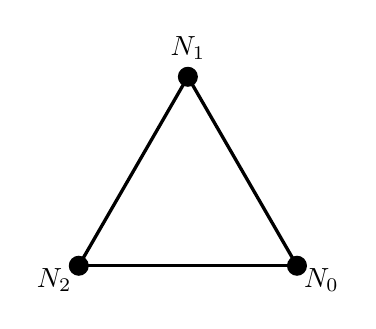
\begin{tikzpicture}[scale=0.8]
                    \foreach \n in {0,...,2}{
                        \draw[very thick] ({-120*\n-30}:2)--({-120*(\n+1)-30}:2) node[midway,sloped,allow upside down]{$\blacktriangleright\blacktriangleright\blacktriangleright$};
                        \draw[fill=black] ({-120*\n-30}:2) circle[radius=0.15];
                    }
                    \draw (-30:2.45) node{$N_0$};
                    \draw (90:2.45) node{$N_1$};
                    \draw (210:2.45) node{$N_2$};
                \end{tikzpicture}
                \caption{Quiver of the $\C^3/\Z_3$ daughter theory.}
                \label{fig:Z3quiver}
            \end{figure}
            The adjacency matrix of this quiver is
            \begin{equation}
                A=
                \begin{bmatrix}
                    0 & 3 & 0 \\
                    0 & 0 & 3 \\
                    3 & 0 & 0
                \end{bmatrix}
            \end{equation}
            which is coherent with the fact that the coefficients of the McKay decomposition of $\rho_1\oplus\rho_1\oplus\rho_1$ are
            \begin{align}
                \begin{split}
                    n_{00} &= 0,\quad n_{01} = 3\qquad n_{02}=0,\\
                    n_{10} &= 0,\quad n_{11} = 0,\qquad n_{12}=3,\\
                    n_{20} &= 3,\quad n_{21} = 0,\qquad n_{22}=0.
                \end{split}
            \end{align}

        \subsubsection{Gauge anomaly cancellation}
        
            We get the three following conditions:
            \begin{align}
                \SU(N_0) &: N_2-N_1 = 0,\\
                \SU(N_1) &: N_0-N_2 = 0,\\
                \SU(N_2) &: N_1-N_0 = 0.
            \end{align}
            which immediately imply
            \begin{equation}
                N_0=N_1=N_2.
            \end{equation}
            From \eqref{eq:sumNiZ3}, we get that $N_0=N_1=N_2=N/3$, meaning that that the daughter theory has quantum gauge symmetry if and only if the parent theory with has gauge group $\SU(N)$ where $N$ is a multiple of $3$. Or, in other words, if the number of D-branes is a multiple of $3$.

    \subsection{Superconformal daughter theories}

        Now that we have discussed the general case and found the resulting field content for an strings an orbifold $\C^3/\Gamma$. The content is then completely determined by the two actions that give ourselves at beginning: 
        \begin{itemize}
            \item the action of $\Gamma$ on $\C^3$ that defines the orbifold per se and dictates how the ``R-symmetry part`` of the projection happens. This action is fixed by the choice of orbifold background we want.
            \item the action of $\Gamma$ on $\C^N$ (from some arbitrary $N$) that defines the embedding of $\Gamma$ in the gauge group $\U(N)$ and and dictates how that ``gauge part'' of the projection happens. Up until, this action was completely arbitrary. In other words, the multiplicities $N_i$ are arbitrary, as long as they sum to $N$, which is arbitrary.
        \end{itemize}
        We discussed in the beginning that the origin the ``gauge part'' of the projection lies in the projection the Chan-Paton factors which was necessary in order to have $\Gamma$-invariant configurations of branes even if they are not at the origin. 
        
        What are the conditions to get a superconformal daughter theory? The answer lies in the choice of the second action, i.e. on the choice of embedding of $\Gamma$ in the gauge group. One can show \cite{vafa1998} that to have conformal invariance, we have to use the regular representation of $\Gamma$. The resulting embedding will be called \emph{regular embedding}. This isonly possible of course if $N=\abs{\Gamma}$. Actually, considering stacks of $N$ branes, we can consider that the rank of the gauge group is $N\abs{\Gamma}$ (we change our $N$) so that the gauge group is $\U(N\abs{\Gamma})$. Recall that the multiplicity of each irredicuble representation in the decomposition of the regular representation is the dimension of the irrep, i.e. $N_i=n_i\equiv\dim\rho_i$ meaning that the gauge group is broken to
        \begin{equation}
            G_{\text{proj}}=\bigotimes_{i\in I}\SU(N n_i)
        \end{equation}
        at low energy. Let us be clear and mention that any choice of multiplicities $N_i$ is valid and gives a supersymmetric daughter theory, but this theory is conformal only if $N_i=n\dim\rho_i$.

        Since the superconformal theories are of particular interest, this case have been studied in some details.

            \subsubsection{Lagrangian}

                Let us describe the lagrangian of the projected theory \cite{vafa1998}. We saw that the gauge group is broken to 
                \begin{equation}
                    G_{\text{proj}}=\bigotimes_{i\in I}\SU(N n_i)
                \end{equation}
                at low energy, with $n_i\equiv\dim\rho_i$. The coupling constant $\tau_i$ (including the theta angle as usual) of the $i$th group is
                \begin{equation}
                    \tau_i=\frac{n_i\tau}{\abs{\Gamma}}
                \end{equation}
                where $\tau$ is the initial $\mN=4$ coupling, or the Type IIB coupling. This implies in particular that
                \begin{equation}
                    \sum_{i\in I}n_i\tau_i=\tau.
                \end{equation}
                There are Yukawa couplings for each triangle of the quiver consisting of two fermionic arrows and a bosonic arrow and quartic scalar interactions for each square consisting of four bosonic arrows. The coefficient ofthese interactions can be by projecting the $\mN=4$ lagrangian in terms of the field we kept. The Yukawa terms are therefore
                \begin{equation}
                    Y=\sum_{i,j,k\in I}\gamma^{f_{ij},f_{jk},f_{kj}}_{ijk}\tr(\psi^{ij}_{f_{ij}}\phi^{jk}_{f_{jk}}\psi^{ki}_{f_{ki}})
                \end{equation}
                and the quartic scalar interaction terms by
                \begin{equation}
                    V=\sum_{i,j,k,l\in I}\eta^{ijkl}_{f_{ij};f_{jk},f_{kl},f_{li}}\tr(\phi^{ij}_{f_{ij}}\phi^{jk}_{f_{jk}}\phi^{kl}_{f_{kl}}\phi^{li}_{f_{li}})
                \end{equation}
                with
                \begin{align}
                    \gamma^{f_{ij},f_{jk},f_{kj}}_{ijk} &= \Gamma_{\alpha\beta,m}(Y_{f_{ij}})\indices{^m_{v_i\bar{v}_j}}(Y_{f_{jk}})\indices{^\beta_{v_j\bar{v}_k}}(Y_{f_{ki}})\indices{^\alpha_{v_k\bar{v}_i}}, \\
                    \eta^{ijkl}_{f_{ij};f_{jk},f_{kl},f_{li}} &= (Y_{f_{ij}})\indices{^{[m}_{v_i\bar{v}_j}}(Y_{f_{jk}})\indices{^{n]}_{v_j\bar{v}_k}}(Y^{f_{kl}})\indices{^{[m}_{v_k\bar{v}_l}}(Y_{f_{li}})\indices{^{n]}_{v_l\bar{v}_i}}.
                \end{align}
                The coefficients $(Y_{f_{ij}})\indices{^\alpha_{v_i\bar{v}_j}}$ and $(Y_{f_{ij}})\indices{^m_{v_i\bar{v}_j}}$ are to be understood as the $f_{ij}$th Clebsch-Gordan coefficients of the projection of $\boldsymbol{4}\otimes\rho_i$ and $\boldsymbol{6}\otimes\rho_i$ onto $\rho_j$, and $\Gamma_{\alpha\beta,m}$ is the invariant in $\boldsymbol{4}\otimes\boldsymbol{4}\otimes\boldsymbol{6}$.
        
                When we choose the regular embedding of $\Gamma$, the 1-loop beta functions have been computed in \cite{vafa1998} and they o indeed vanish \cite{vafa1998}.
                
                In the same paper, the superpotential inherited from the parent theory is shown to be
                \begin{equation}
                    \mathcal{W}=\sum_{i,j,k\in I}\sum_{f_{ij},f_{jk},f_{ki}}h^{f_{ij},f_{jk},f_{kj}}_{ijk}\tr(\phi^{ij}_{f_{ij}}\phi^{jk}_{f_{jk}}\phi^{ki}_{f_{ki}})
                \end{equation}
                where
                \begin{equation}
                    h^{f_{ij},f_{jk},f_{kj}}_{ijk} = \eps_{\alpha\beta\gamma}(Y_{f_{ij}})\indices{^\alpha_{v_i\bar{v}_j}}(Y_{f_{jk}})\indices{^\beta_{v_j\bar{v}_k}}(Y_{f_{ki}})\indices{^\gamma_{v_k\bar{v}_i}}
                \end{equation}
                and $(Y_{f_{ij}})\indices{^\alpha_{v_i\bar{v}_j}}$ is now the $f_{ij}$th Clebsch-Gordan coefficient of the projection of $\boldsymbol{3}\otimes\rho_i$ onto $\rho_j$.


    \subsection{Fractional branes}\todo{Rework/understand this section}
        
        We saw that invariant configurations of D-branes naturally give rise to the regular representation of the orbifold group $\Gamma$ on the Chan-Paton factors. Correspondingly, these branes are called $\emph{regular branes}$. The regular representation is not irreducible and it decomposes as
        \begin{equation}
            \rho_{\text{reg}}=\bigoplus_{i\in I} N_i\rho_i
        \end{equation}
        with $N_i=\dim\rho_i$ in terms of the irreducible representations of $\Gamma$. One may then wonder about the existence of a more ``elementary'' set of D-branes such that the open strings attached to the latter carry Chan-Paton factors indices that transform in an irreducible representation. Those indeed do exist and are called \emph{fractional D-branes}. They are BPS object that carry only a fraction of the charge with respect to the untwisted RR $(p+1)$-form of a regular brane but they are charged with respect to some twisted RR $(p+1)$-form, contrarily to the regular D-branes. They are stuck at the orbifold fixed point (where all twisted fields sit) since sitting elsewhere would require an invariant configuration in the covering space and those correspond to the regular representation, as we mentioned. So they cannot be fractional D-branes.

        An important property of fractional D-branes is that they can be interpreted as higher-dimensional branes wrapped on exceptional cycles of the resolved space. In the orbifold limit, these exceptional cycles collapses leaving lower-dimensional fractional branes behind. This suggest a link between the spectrum of the D-branes and the homology of the resolved orbifold space. More precisely, it is linked to its homological K-theory. This is has been studied a lot.
    
        From the point of view of boundary conformal field theory\footnote{CFT on a manifold with boundary. Boundary conditions for open strings are interpreted as coherent states of the corresponding closed string 2d CFT.}, \emph{fractional D-branes} are reflected by boundary states in twisted sectors.

    \subsection{A note on $(p+1)$-dimensional quiver gauge theories}

        Let us mention that we can generalize our initial brane-world paradigm and consider D$p$-branes in type II string theory (type IIA if $p$ is even and type IIB if $p$ is odd) instead of just D$3$-branes. The spacetime is then of the form
        \begin{equation}
            M = \R^{1,p}\times\R^{9-p}/\Gamma
        \end{equation}
        where $\Gamma$ is a discrete subgroup of $\Spin(9-p)$. If $\Gamma$ is a subgroup of a special holonomy group, we recover a somewhat generalized version of the paradigm that we discussed above. In this case the transverse space is a Calabi-Yau orbifold and some degree of supersymmetry is preserved. Note that the fermionic and bosonic quivers that coincides. If $\Gamma$ is not a subgroup of a special holonomy group, then the $(p+1)$-dimensional quiver gauge theory that we obtain in the low-energy limit is not supersymmetric. We then have different quivers for the fermions and the bosons, although with the same vertices, by definition.

        Recall that the fraction of supercharges that is preserved by compactifying on a Calabi-Yau $n$-fold (with $\SU(n)$ holonomy) is $2^{1-n}$. Starting from the $\mN=2$ 10-dimensional type IIB string theory with 32 supercharges, this means that
        \begin{itemize}
            \item if we compactify on a $1$-fold, we get $32$ supercharges in $8$ dimensions so $\mN=2$,
            \item if we compactify on a $2$-fold, we get $16$ supercharges in $6$ dimensions so $\mN=2$,
            \item if we compactify on a $3$-fold, we get $8$ supercharges in $4$ dimensions so $\mN=2$,
            \item is we compactify on a $4$-fold, we get $4$ supercharges in $2$ dimensions so $\mN=4$.
        \end{itemize}

        We will however mostly mostly consider $4$-dimensional quiver gauge theories, i.e. living on D$3$-branes.

\section{$\mN=2$ daughter theories}\label{sec:N2QGT}

    %Let us consider that $\Gamma$ is a finite subgroup of $\SU(2)\subset\SU(3)$. It naturally acts on $\C^3$ trough its fundamental representation $\bs{2}$ as $\bs{1}\oplus\bs{2}$ (only acts on 2 coordinates).

    \subsection{$S=\C\times\C^2/\Z_n$}

        We consider a representation $(\rho,\C^N)$ of $\Z_n$. We decompose it on the set of irreducible representations of $\Z_n$ as
        \begin{equation}
            (\rho,\C^n)=\bigoplus^{n-1}_{i=0}N_i(\rho_i,\C).
        \end{equation}
        In other words, it is equivalent to the representation
        \begin{equation}
            \rho(g)=
            \begin{bmatrix}
                1 & & & \cdots & & & 0 \\
                & \ddots & & & & & \\
                & & 1 & & & &  \\
                \vdots & & & \ddots & & & \vdots \\
                & & & & \zeta^{n-1}_n & & \\
                & & & & & \ddots & \\
                0 & & & \cdots & & & \zeta^{n-1}_n 
            \end{bmatrix}
            \hspace{-0.2cm}
            \begin{tabular}{l}
            $\left.\lefteqn{\phantom{
                \begin{matrix}
                    a_0\\ \ddots\\ a_0\ 
                \end{matrix} 
            }}\right\}N_0$\\
            \vdots \\
            $\left.\lefteqn{\phantom{
                \begin{matrix}
                    b_0\\ \ddots\\ b_0\ 
                \end{matrix}
            }} \right\}N_{n-1}$
            \end{tabular}.\label{eq:reprrhoZn}
        \end{equation}
        Since $\dim\rho_i=1$, $\sum_i N_i=N$. 

        The gauge field configurations that are left invariant under the action of $\Z_n$ are therefore the ones that satisfy
        \begin{equation}
            \rho(g)A_\mu\rho(g)^{-1}=A_\mu.
        \end{equation}
        The constrained is easily solved by using the bi-index notation:
        \begin{equation}
            A_{\mu;i\alpha_i,i\beta_j}\mapsto \rho_i(g)A_{\mu;i\alpha_i,j\beta_j}\rho_j(g)^{-1}=\zeta^{i-j}_nA_{\mu;i\alpha_i,j\beta_j}.
        \end{equation}
        thus only the configurations with $A_{\mu;i\alpha_i,j\beta_j}=0$ if $i\neq j$ are invariant. The gauge field has therefore a block diagonal form:
        \begin{equation}
            A_\mu=
            \begin{bmatrix}
                A_{\mu;00} & & & \\
                & A_{\mu;11} & & \\
                & & \ddots & \\
                & & & A_{\mu;n-1,n-1}
            \end{bmatrix}
        \end{equation}
        with $A_{\mu;ij}\equiv (A_{\mu;i\alpha_i,j\beta_j})_{\alpha_i=0,\dots,N_i,\beta_j=0,\dots,N_j}$. The block $A_{ii}$ transforms under $\Z_n$ as $(\rho_i,V_i)^{N_i}$. For now it is only a simple generalization of the case $\C^3/\Z_3$. This makes sense: projection of the gauge field only depends the discrete group $\Gamma$, not on the way it acts on $\C^3$ because it does not transform under R-symmetry.
        
        The gauge group is now broken to
        \begin{equation}
            G_{\text{proj}}=\prod^{n-1}_{i=0}~\U(N_i).
        \end{equation}

        Now for the scalar fields. The action of $\Z_n$ that we consider leaves the first component of $\C^3$ untouched so we take the action $\boldsymbol{1}\oplus\boldsymbol{2}$ where $\boldsymbol{2}$ is the usual action of $\Z_n$ on $\C^2$. In other words, 
        \begin{equation}
            R(g)=
            \begin{bmatrix}
                1 & 0 & 0 \\
                0 & \zeta_n & 0 \\
                0 & 0 & \zeta^{-1}_n
            \end{bmatrix}.
        \end{equation}
        Or, equivalently, $R(g)\indices{^m_n}=\delta\indices{^m_n}A_n$ with $A_m=(1,1,\zeta_n,\zeta_n,\zeta^{-1}_n,\zeta^{-1}_n)$. The scalar field configurations that are left invariant satisfy
        \begin{equation}
            R(g)\indices{^m_n}\rho(g)X^n\rho(g)^{-1}=X^m
        \end{equation}
        for all $g\in\Z_n$. Using the bi-index notations, this becomes
        \begin{align}
            X^m_{i\alpha_i,j\beta_j}\mapsto  \delta\indices{^m_n}A_n\rho_i(g)X^m_{i\alpha_i,j\beta_j}\rho_j(g)^{-1}  = \delta\indices{^m_n}A_n\zeta^{i-j}_n X^m_{i\alpha_i,j\beta_j} =
            \begin{cases}
                \zeta^{i-j}_nX^m_{i\alpha_i,j\beta_j},\quad m=0,1\\
                \zeta^{i-j+1}_nX^m_{i\alpha_i,j\beta_j},\quad m=2,3\\
                \zeta^{i-j-1}_nX^m_{i\alpha_i,j\beta_j},\quad m=4,5\\
            \end{cases}\\
            \bar{X}^m_{i\alpha_i,j\beta_j}\mapsto \delta\indices{^m_n}\bar{A_n}\rho_i(g)\bar{X}^m_{i\alpha_i,j\beta_j}\rho_j(g)^{-1}  = \delta\indices{^m_n}\bar{A_n}\zeta^{i-j}_n X^m_{i\alpha_i,j\beta_j} =
            \begin{cases}
                \zeta^{i-j}_nX^m_{i\alpha_i,j\beta_j},\quad m=0,1\\
                \zeta^{i-j-1}_nX^m_{i\alpha_i,j\beta_j},\quad m=2,3\\
                \zeta^{i-j+1}_nX^m_{i\alpha_i,j\beta_j},\quad m=4,5\\
            \end{cases}
        \end{align}
        thus only the configurations with $X^{0,1}_{i\alpha_i,j\beta_j}=0$ if $i-j\neq0$, $X^{2,3}_{i\alpha_i,j\beta_j}=0$ if $i-j+1\neq0$ and $X^{4,5}_{i\alpha_i,j\beta_j}=0$ if $i-j-1\neq0$ are left invariant (and similarly for the conjugated fields). The scalar fields $X$ have a the following forms:
        {\small
        \begin{align}
            X^{0,1}&=
            \begin{bmatrix}
                X^{0,1}_{00} &  & 0 \\
                 & \ddots & \\
                0 & & X^{0,1}_{n-1,n-1}
            \end{bmatrix},\\
            X^{2,3}&=
            \begin{bmatrix}
                0 & X^{2,3}_{01} & & 0 \\
                 & \ddots & \ddots & \\
                 & & 0 & X^{2,3}_{n-2,n-1} \\
                X^{2,3}_{n-1,0} & & & 0 
            \end{bmatrix},\quad
            X^{4,5}=
            \begin{bmatrix}
                0 & & & X^{4,5}_{0,n-1} \\
                X^{4,5}_{10} & 0 & & \\
                 & \ddots & \ddots  & \\
                0 & & X^{4,5}_{n-1,n-2} & 0
            \end{bmatrix},\\
            \bar{X}^{0,1}&=
            \begin{bmatrix}
                \bar{X}^{0,1}_{00} &  & 0 \\
                 & \ddots & \\
                0 & & \bar{X}^{0,1}_{n-1,n-1}
            \end{bmatrix},\\
            \bar{X}^{2,3}&=
            \begin{bmatrix}
                0 & & & \bar{X}^{2,3}_{0,n-1} \\
                \bar{X}^{2,3}_{10} & 0 & & \\
                 & \ddots & \ddots  & \\
                0 & & \bar{X}^{2,3}_{n-1,n-2} & 0
            \end{bmatrix},\quad
            \bar{X}^{4,5}=
            \begin{bmatrix}
                0 & \bar{X}^{4,5}_{01} & & 0 \\
                 & \ddots & \ddots & \\
                 & & 0 & \bar{X}^{4,5}_{n-2,n-1} \\
                 \bar{X}^{4,5}_{n-1,0} & & & 0
            \end{bmatrix}
        \end{align}}
        so $X^m_{ij}$ is an $N_i\times N_j$ block and transforms under the representation $(\boldsymbol{\textbf{N}_i},\boldsymbol{\bar{\textbf{N}}_j})$ of $\U(N_i)\times\U(N_j)$:
        \begin{align}
            X^{0,1}_{i,i} &\in \boldsymbol{\textbf{N}_i}\otimes\boldsymbol{\bar{\textbf{N}}_i} \cong \Hom(V_i,V_i),\\
            X^{2,3}_{i,i+1} &\in \boldsymbol{\textbf{N}_{i+1}}\otimes\boldsymbol{\bar{\textbf{N}}_i} \cong \Hom(V_{i+1},V_i),\\
            X^{4,5}_{i+1,i} &\in \boldsymbol{\textbf{N}_i}\otimes\boldsymbol{\bar{\textbf{N}}_{i+1}} \cong \Hom(V_i,V_{i+1}).
        \end{align}
        So the scalar fields are split up in three families depending on the way they transform under R-symmetry. We now see a big difference with the case $\C^3/\Z_3$: since the R-symmetry does not act the same way on each directions in $\C^3$, the invariant scalar field configurations are not the same in each direction either.

        Let us draw the quiver for the case $n=3$ so that we can compare to \ref{fig:Z3quiver}. We have $2\cdot 9=18$ real scalar fields in $9$ different representations:
        \begin{align}
            X^0_{00},X^1_{00}&\in(\boldsymbol{\textbf{N}_0},\boldsymbol{\bar{\textbf{N}}_0}),\quad
            X^0_{11},X^1_{11}\in(\boldsymbol{\textbf{N}_1},\boldsymbol{\bar{\textbf{N}}_1}),\quad
            X^0_{22},X^1_{22}\in(\boldsymbol{\textbf{N}_2},\boldsymbol{\bar{\textbf{N}}_2}),\\
            X^2_{01},X^3_{01}&\in(\boldsymbol{\textbf{N}_1},\boldsymbol{\bar{\textbf{N}}_0}),\quad
            X^2_{12},X^3_{12}\in(\boldsymbol{\textbf{N}_2},\boldsymbol{\bar{\textbf{N}}_1}),\quad
            X^2_{20},X^3_{20}\in(\boldsymbol{\textbf{N}_0},\boldsymbol{\bar{\textbf{N}}_2}),\\
            X^4_{10},X^5_{10}&\in(\boldsymbol{\textbf{N}_0},\boldsymbol{\bar{\textbf{N}}_1}),\quad
            X^4_{21},X^5_{21}\in(\boldsymbol{\textbf{N}_1},\boldsymbol{\bar{\textbf{N}}_2}),\quad
            X^4_{02},X^5_{02}\in(\boldsymbol{\textbf{N}_2},\boldsymbol{\bar{\textbf{N}}_0}),
        \end{align}
        We now only have 1 complex scalar in each representation and the quiver is given by \ref{fig:2Z3quiver}.
        \begin{figure}[H]
            \centering
            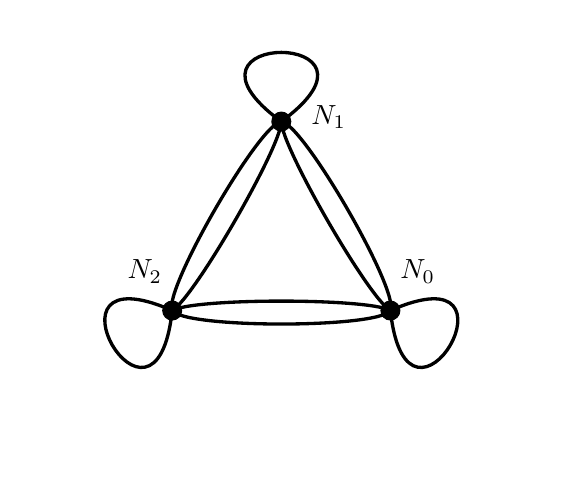
\begin{tikzpicture}[scale=0.8]
                \foreach \n in {0,...,2}{
                    \draw[very thick] ({120*\n-30}:2) .. controls ({120*\n-20}:2) and ({120*\n+120-40}:2) .. ({120*\n+120-30}:2) node[midway,sloped,allow upside down]{$\blacktriangleright$};
                    \draw[very thick] ({120*\n-30}:2) .. controls ({120*\n-30}:1.6) and ({120*\n+120-30}:1.6) .. ({120*\n+120-30}:2) node[midway,sloped,allow upside down]{$\blacktriangleleft$};
                    \draw[very thick] ({120*\n-30}:2) .. controls ({120*\n}:4) and ({120*\n-60}:4) .. ({120*\n-30}:2) node[midway,sloped,allow upside down]{$\blacktriangleright$};
                    \draw[fill=black] ({120*\n-30}:2) circle[radius=0.15];
                }
                \draw (-10:2.2) node{$N_0$};
                \draw (70:2.2) node{$N_1$};
                \draw (190:2.2) node{$N_2$};
            \end{tikzpicture}
            \caption{Quiver of the $\C\times\C^2/\Z_3$ daughter theory.}
            \label{fig:2Z3quiver}
        \end{figure}
        It is easy to see how the construction of the the quiver generalizes for arbitrary $n$. The adjacency matrix is
        \begin{equation}
            A=
            \begin{bmatrix}
                1 & \cdots & 1 \\
                \vdots & \ddots & \vdots \\
                1 & \cdots & 1
            \end{bmatrix}
        \end{equation}
        which is, as it should, coincides with the McKay decomposition of $\boldsymbol{1}\oplus\boldsymbol{2}$:
        \begin{align}
            \begin{split}
                n_{00} &= 1,\quad\dots,\qquad n_{0,n-1}=1,\\
                &\vdots\hspace{3.7cm}\vdots\\
                n_{n-1,0} &= 1,\quad\dots,\qquad n_{n-1,n-1}=1.
            \end{split}
        \end{align}
        
        Gauge anomaly cancellation now imposes that
        \begin{equation}
            N_{i-1}-N_{i-1}+N_{i+1}+N_{i+1}=0
        \end{equation}
        for $i=0,\dots,n-1$. Those constrains are always satisfied so the the factors $N_i$ are arbitrary, as long as $\sum_iN_i=N$ of course.

        This quiver is easy to scale up for any $n$. We therefore implement that into Mathematica and get the quivers for any $n$.

    \subsection{$S=\C\times\C^2/\D_n$}

        We quotient $\C^3$ by the binary dihedral group $\D_n$ that acts on the last two components. This group is geneated by two elements that we denote $A$ and $B$. Firther details on its structure and representations are given in appendix \ref{app:su2subgroups}. A set of irreducible representations of $\D_n$ is given by
        \begin{equation}
            \{(\rho_i,V_i)\}_{i=0,\dots,n+2}
        \end{equation}
        with $V_i=\C$ for $i=0,\dots,3$ and $V_i=\C^2$ for $i=4,\dots,n+2$, so there are $4$ one-dimensional representations and $n-1$ two-dimensional representations. It is more convenient to treat the $1$-dimensional and $2$-dimensional representations idependently. We therefore denote by $\sigma_i$ with $i=0,\dots,3$ the $1$-dimensional representations and by $\mu_r$ with $r=1,\dots,n-1$ the $2$-dimensional ones:
        \begin{equation*}
        \begin{array}{cc}
            \multirow{7}{*}{$\begin{array}{|c|c|c|}
                \hline
                a & \sigma_a(A) & \sigma_a(B) \text{ ($n$ even or odd)} \\
                \hline
                0 & 1 & 1\\ \hline
                1 & 1 & -1 \\ \hline
                2 & -1 & 1 \text{ or } i \\ \hline
                3 & -1 & -1 \text{ or } -i \\
                \hline
            \end{array}$} & \\
            & {\hspace{0.9cm}\mu_r(A) = 
            \begin{bmatrix}
                e^{i\frac{\pi}{n}r} & 0\\
                0 & e^{-i\frac{\pi}{n}r} 
            \end{bmatrix}}\\
            & \\
            & {\rho_r(B) = 
            \begin{bmatrix}
                0 & -1 \\
                1 & 0
            \end{bmatrix}}
        \end{array}
        \end{equation*}
        We note that there is a slight difference for the $1$-dimensional representations if $n$ is even or odd.
        
        Any representation of $(\rho,\C^N)$ of $\D_n$ can be decomposed as
        \begin{equation}
            (\rho,\C^n) = \left( \bigoplus^3_{a=0}(\sigma_a,\C) \right)\oplus\left( \bigoplus^{n-1}_{r=1}(\mu_r,\C^2) \right).
        \end{equation}
        The invariant gauge field configurations were found to be of the form
        \begin{equation}
            A_\mu=
            {\tiny
            \left[
            \begin{array}{*{20}c}
                \times & 0 & 0 & 0 & & & & & & \cdots & 0 \\
                0 & \times & 0 & 0 & & & & & & & \\
                0 & 0 & \times & 0 & & & & & & & \\
                0 & 0 & 0 & \times & & & & & & & \\
                & & & & x_1 & 0 & & & & & \\
                & & & & 0 & -x_1 & & & & & \\
                & & & & & & x_2 & 0 & & & \\
                & & & & & & 0 & -x_2 & & & \\
                \vdots & & & & & & & & \ddots & & \vdots \\
                & & & & & & & & & x_{n-1} & 0 \\
                0 & & & & & & & & & 0 & -x_{n-1}
        \end{array}
        \right]}.\label{eq:invformAmuDn}
        \end{equation}
        where each entry $(i,j)$ is an arbitrary block of size $N_i\times N_j$. The explicit derivations are carried out in appendix \ref{app:invconfDn}. The projected gauge group is then
        \begin{equation}
            G_{\text{proj}} = \SU(N_0)\times\dots\SU(N_3)\times\SU(2N_4)\times\dots\times\SU(2N_{n+3}).
        \end{equation}


        %The invariant scalar field configurations are computed to be of the form
        %\begin{equation}
        %    X^m=
        %    {\tiny
        %    \left[
        %    \begin{array}{*{20}c}
        %        \times & 0 & 0 & 0 & & & & & & \cdots & 0 \\
        %        0 & \times & 0 & 0 & & & & & & & \\
        %        0 & 0 & \times & 0 & & & & & & & \\
        %        0 & 0 & 0 & \times & & & & & & & \\
        %        & & & & x_1 & 0 & & & & & \\
        %        & & & & 0 & -x_1 & & & & & \\
        %        & & & & & & x_2 & 0 & & & \\
        %        & & & & & & 0 & -x_2 & & & \\
        %        \vdots & & & & & & & & \ddots & & \vdots \\
        %        & & & & & & & & & x_{n-1} & 0 \\
        %        0 & & & & & & & & & 0 & -x_{n-1}
        %\end{array}
        %\right]}\label{eq:invformXmDn}
        %\end{equation}
        It is interesting to notice the main differences with the case of $\Z_n$:
        \begin{itemize}
            \item since $2\D_n$ is not abelian, it can have irreps of two or more dimension (which it does). This implies that the gauge field bloacks $A_{\mu;ij}$ are not necessarily diagonal. This will have important consequence for the residual gauge group.
            \item again because some irreps are mode then $1$-dimensional, we can act on $\C^3$ with non-diagonal actions (which we do). This means that components of the different complex scalars can be exchanged under R-symmetry.
        \end{itemize}


        As we mentioned previously, there is no constrain on the ranks of the gauge groups coming from the the anomaly condition, it is automatically anomaly-free.

    \subsection{$S=\C\times\C^2/\T,\mathcal{O},\I$}

        \todo{Continue.}




\section{$\mN=1$ daughter theories}

    \subsection{$S=\C^3/\Z_n$}

        Let us now consider the general case of $\Z_n$ acting on $\C^3$, i.e. we want to generalize the case that we treated in section \ref{sec:C3Z3}. 
        
        \subsubsection{Actions of $\Z_n$ on $\C^3$}
        
            The first thing to do is to specify a representation of $\Z_n$ on $\C^3$. Any representation $(R,\C^3)$ can be decomposed as
            \begin{equation}
                R=\bigoplus^{n-1}_{k=0} \rho^{\oplus n_k}_k
            \end{equation}
            and is therefore equivalent to a block-diagonal representation. This implies that $\sum_kn_k=3$ so $R$ can always be written as
            \begin{equation}
                R(g)= (\rho_a\oplus\rho_b\oplus\rho_c)(g)=
                \begin{bmatrix}
                    \zeta^a_n & 0 & 0 \\
                    0 & \zeta^b_n & 0 \\
                    0 & 0 & \zeta^c_n
                \end{bmatrix}\label{eq:reprZnC3}
            \end{equation}
            with $a,b,c$ some arbitrary exponents. We denote the representation \eqref{eq:reprZnC3} by $(a,b,c)$. Let us make a few remarks on these representations:
            \begin{itemize}
                \item Since we consider $\Z_n$ as a subgroup of $\SU(3)$, we must have
                \begin{equation}
                    (a+b+c)\mod n = 0\label{eq:cdtabc}
                \end{equation}
                such that $\det(R(g))=1$.
                \item Taking $a$ or $a+n$ gives the same representation and the same is true for $b$ and $c$, so we we can actually restrict ourselves to $0<a,b,c<n$. We can trade the strict inequalities and allow the values $0$ or $n$ if we want to consider trivial representations as well. In this case, we will find that at least one direction of $\C^3$ is left untouched, i.e. we are in the situation where the orbifold is actually $\C\times\C^2/\Z_n$, which we will not consider here.
                \item Permuting $a,b,c$ gives equivalent representations so we can take $a,b,c$ to be ordered, so $0<a\leq b\leq c<n$.
            \end{itemize}

            The problem has now been reformulated as follows:
            we are looking for all possible ordered triplets $(a,b,c)$ such that $0<a\leq b\leq c<n$ and \eqref{eq:cdtabc}. For $n=1$ and $n=2$, it is clear that this is not possible, the possibilities involve at least one trivial representation. For $n=3$, the only possibility is $(1,1,1)$, the one we used in \ref{sec:C3Z3}. What about bigger values of $n$? First, note that $0<a\leq b\leq c<n$ implies that the maximum value of $a+b+c$ is $3n-1$. From equation \eqref{eq:cdtabc}, the only two possibilities are then $a+b+c=n$ or $a+b+c=2n$. What simplifies the analysis is that the second case can actually be ignored because it is already being taken care of by the first case. Let us explain that in more details: \todo{details}.
            
            Now that we have seen that the only possibility is $a+b+c=n$, we find that the maximum value that $a$ can take is $\lfloor n/3\rfloor$, so $a=1,\dots,\lfloor n/3\rfloor$. $c$ can then be expressed in terms of $a$ and $b$ as $c=n-a-b$. The constraint $b\leq c$ then implies $b\leq (n-a)/2$, i.e. $b=a,\dots,\lfloor (n-a)/2\rfloor$. To summarize, the representations are all the representations of the form
            \begin{equation}
                (a,b,n-a-b)
            \end{equation}
            with $a=1,\dots,\lfloor n/3\rfloor$ and $b=a,\dots,\lfloor (n-a)/2\rfloor$. For small values, we get
            \begin{align*}
                \Z_1 &: \text{necessarily involves a trivial representation}\\
                \Z_2 &: \text{necessarily involves a trivial representation}\\
                \Z_3 &: (1,1,1)\\
                \Z_4 &: (1,1,2)\\
                \Z_5 &: (1,1,3),(1,2,2)\label{reprZ5C3}\\
                \Z_6 &: (1,1,4),(1,2,3),(2,2,2)\\
                \Z_7 &: (1,1,5),(1,2,4),(1,3,3),(2,2,3)\\
                &\vdots
            \end{align*}
            \todo{Correct this.}
            For an arbitrary $n$, the total number of different representation is
            \begin{equation}
                \sum^{\lfloor n/3\rfloor}_{a=1}~\left\lfloor \frac{n-3a}{2}+1\right\rfloor = \begin{cases}
                    3k^2,\qquad\text{if $n=6k$}\\
                    3k^2+k,\qquad\text{if $n=6k+1$},\\
                    3k^2+2k,\qquad\text{if $n=6k+2$},\\
                    3k^2+3k+1,\qquad\text{if $n=6k+3$},\\
                    3k^2+4k+1,\qquad\text{if $n=6k+4$},\\
                    3k^2+5k+2,\qquad\text{if $n=6k+5$}
                \end{cases}
            \end{equation}
            The details are presented in appendix \ref{app:compsum}.

        \subsubsection{Example: $\Z_5$}

            For $\Z_5$, we saw that there are two nonequivalent ways of acting on $\C^3$, see \eqref{reprZ5C3}. Let us first consider the action $(1,1,3)$
            \begin{equation}
                R(g)=
                \begin{bmatrix}
                    \zeta_5 & 0 & 0\\
                    0 & \zeta_5 & 0\\
                    0 & 0 & \zeta^3_5
                \end{bmatrix}
            \end{equation}
            i.e. $R=\rho_1\oplus\rho_1\oplus\rho_3$.

            For the gauge field, the reasoning is exactly the same than for $\Z_3$ and we get
            \begin{equation}
                A_\mu=
                \begin{bmatrix}
                    A_{\mu;00} & & \\
                    & \ddots & \\
                    & & A_{\mu;44}
                \end{bmatrix}
            \end{equation}
            where each block $A_{\mu;ii}$ is of size $N_i\times N_i$. The projected gauge group is
            \begin{equation}
                G_{\text{proj}} = \U(N_0)\times\U(N_1)\times\U(N_2)\times\U(N_3)\times\U(N_4).
            \end{equation}

            The scalar fields transform as
            \begin{equation}
                X^m_{i\alpha_i,j\beta_j}\to R(g)\indices{^m_n}\rho_i(g)X^n_{i\alpha_i,j\beta_j}\rho_j(g)^{-1}
            \end{equation}
            so the invariant configurations must satisfy
            \begin{equation}
                X^m_{i\alpha_i,j\beta_j} = R(g)\indices{^m_n}\zeta^{i-j}_4\rho_i(g)X^n_{i\alpha_i,j\beta_j} = 
                \begin{cases}
                    \zeta^{i-j+1}X^m_{i\alpha_i,j\beta_j},\quad\text{if } m=0,1,2,3\\
                    \zeta^{i-j+3}X^m_{i\alpha_i,j\beta_j},\quad\text{if } m=4,5.
                \end{cases}
            \end{equation}
            and are therefore of the form
            \begin{equation}
                X^m = 
                \begin{bmatrix}
                    0 & X^m_{01} & 0 & 0 & 0\\
                    0 & 0 & X^m_{12} & 0 & 0\\
                    0 & 0 & 0 & X^m_{23} & 0\\
                    0 & 0 & 0 & 0 & X^m_{34}\\
                    X^m_{40} & 0 & 0 & 0 & 0
                \end{bmatrix}
            \end{equation}
            for $m=0,1,2,3$ and 
            \begin{equation}
                X^m = 
                \begin{bmatrix}
                    0 & 0 & 0 & X^m_{03} & 0\\
                    0 & 0 & 0 & 0 & X^m_{14}\\
                    X^m_{20} & 0 & 0 & 0 & 0\\
                    0 & X^m_{31} & 0 & 0 & 0\\
                    0 & 0 & X^m_{42} & 0 & 0
                \end{bmatrix}
            \end{equation}
            for $m=4,5$. Gauge anomaly cancellation imposes
            \begin{align}
                -N_{i-2}+N_{i+2}-2N_{i+1}+2N_{i-1}=0
            \end{align}
            for $i=0,1,2,3,4$ which implies that
            \begin{equation}
                N_0=N_1=N_2=N_3=N_4.
            \end{equation}

            Now if we choose the representation $(1,2,2)$, i.e.
            \begin{equation}
                R(g)=
                \begin{bmatrix}
                    \zeta_5 & 0 & 0\\
                    0 & \zeta^2_5 & 0\\
                    0 & 0 & \zeta^2_5
                \end{bmatrix}
            \end{equation}
            we get instead that the invariant field configurations must satisfy
            \begin{equation}
                X^m_{i\alpha_i,j\beta_j} = R(g)\indices{^m_n}\zeta^{i-j}_4\rho_i(g)X^n_{i\alpha_i,j\beta_j} =
                \begin{cases}
                    \zeta^{i-j+1}X^m_{i\alpha_i,j\beta_j},\quad\text{if } m=0,1\\
                    \zeta^{i-j+2}X^m_{i\alpha_i,j\beta_j},\quad\text{if } m=2,3,4,5.
                \end{cases}
            \end{equation}
            and are therefore of the form
            \begin{equation}
                X^m = 
                \begin{bmatrix}
                    0 & X^m_{01} & 0 & 0 & 0\\
                    0 & 0 & X^m_{12} & 0 & 0\\
                    0 & 0 & 0 & X^m_{23} & 0\\
                    0 & 0 & 0 & 0 & X^m_{34}\\
                    X^m_{40} & 0 & 0 & 0 & 0
                \end{bmatrix}
            \end{equation}
            for $m=0,1$ and 
            \begin{equation}
                X^m = 
                \begin{bmatrix}
                    0 & 0 &  X^m_{02} & 0 & 0\\
                    0 & 0 & 0 &  X^m_{13} & 0\\
                    0 & 0 & 0 & 0 &  X^m_{24}\\
                    X^m_{30} & 0 & 0 & 0 & 0\\
                    0 &  X^m_{41} & 0 & 0 & 0
                \end{bmatrix}
            \end{equation}
            for $m=2,3,4,5$. Gauge anomaly cancellation imposes
            \begin{align}
                -2N_{i+2}+2N_{i-2}-N_{i+1}+N_{i-1}=0
            \end{align}
            for $i=0,1,2,3,4$ which implies that
            \begin{equation}
                N_0=N_1=N_2=N_3=N_4.
            \end{equation}
            \todo{Right conditions?}

            \begin{figure}
                \centering
                \begin{subfigure}[b]{0.3\textwidth}
                    \centering
                    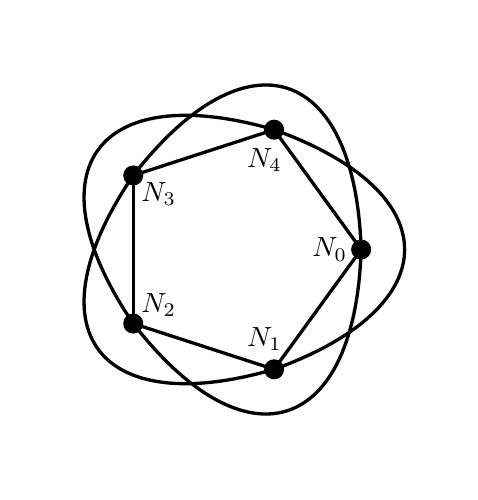
\begin{tikzpicture}[scale=0.8]
                        \foreach \n in {0,...,4}{
                            \draw[very thick] (-72*\n:2) .. controls ({-72*(\n+1)+15}:3.5) and ({-72*(\n+1)-15}:3.5) .. ({-72*(\n+2)}:2) node[midway,sloped,allow upside down]{$\blacktriangleright$};
                            \draw[very thick] ({-72*\n}:2) -- ({-72*(\n-1)}:2) node[midway,sloped,allow upside down]{$\blacktriangleright\blacktriangleright$};
                            \draw[fill=black] (-72*\n:2) circle[radius=0.15];
                            \draw (-72*\n:1.5) node{$N_\n$};
                        }
                    \end{tikzpicture}
                    \caption{$(1,1,3)$}
                    \label{fig:y equals x}
                \end{subfigure}
                \hspace{2cm}
                \begin{subfigure}[b]{0.3\textwidth}
                    \centering
                    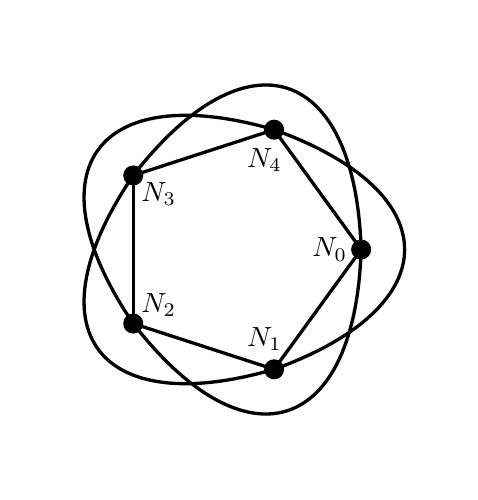
\begin{tikzpicture}[scale=0.8]
                        \foreach \n in {0,...,4}{
                            \draw[very thick] (-72*\n:2) .. controls ({-72*(\n+1)+15}:3.5) and ({-72*(\n+1)-15}:3.5) .. ({-72*(\n+2)}:2) node[midway,sloped,allow upside down]{$\blacktriangleleft\blacktriangleleft$};
                            \draw[very thick] ({-72*\n}:2) -- ({-72*(\n-1)}:2) node[midway,sloped,allow upside down]{$\blacktriangleright$};
                            \draw[fill=black] (-72*\n:2) circle[radius=0.15];
                            \draw (-72*\n:1.5) node{$N_\n$};
                        }
                    \end{tikzpicture}
                    \caption{$(1,2,2)$}
                    \label{fig:three sin x}
                \end{subfigure}
                \caption{Quivers of the $\C^3/\Z_5$ daughter theories.}
                \label{fig:Z5graphs}
           \end{figure}

           Note that, even we thought that $(1,1,3)$ and $(1,2,2)$ were different representation, that are actually equivalent in the sense that $(1,1,3)+(1,1,3)=(2,2,1)$. The two quivers in fig. \ref{fig:Z5graphs} should therefore be the same. And indeed, upon further inspection, the two are the same. To see this, we can rename the vertices in the second graph as $N_1\to N_3,N_2\to N_1,N_3\to N_4,N_4\to N_2$. This renaming defines the bijection between the two graphs. A more pragmatic way to see this is to look at the adjacency matrices:
           \begin{equation}
                a_{(1,1,3)}=
                \begin{bmatrix}
                    0 & 0 & 1 & 0 & 2 \\
                    2 & 0 & 0 & 1 & 0 \\
                    0 & 2 & 0 & 0 & 1 \\
                    1 & 0 & 2 & 0 & 0 \\
                    0 & 1 & 0 & 2 & 0
                \end{bmatrix}\qquad
                a_{(1,2,2)}=
                \begin{bmatrix}
                    0 & 0 & 0 & 2 & 1 \\
                    1 & 0 & 0 & 0 & 2 \\
                    1 & 1 & 0 & 0 & 0 \\
                    0 & 2 & 1 & 0 & 0 \\
                    0 & 0 & 2 & 1 & 0
                \end{bmatrix}.
           \end{equation}
           Changing the names of the vertices is equivalent to swapping line and columns. For example, 

        \subsubsection{General $\Z_n$}

           Let us now consider the general action
           \begin{equation}
                R(g)=
                \begin{bmatrix}
                    \zeta^a_n & 0 & 0\\
                    0 & \zeta^b_n & 0\\
                    0 & 0 & \zeta^c_n
                \end{bmatrix}
           \end{equation}
           of $\Z_n$ on $\C^3$, where $(a,b,c)$ one of the representation that we studied before. In particular, recall that $a+b+c=n$. Following the same reasoning than before, we get that the gauge field of of the form
           \begin{equation}
               A_\mu=
               \begin{bmatrix}
                   A_{\mu;00} & & \\
                   & \ddots & & \\
                   & & A_{\mu;n-1,n-1}
               \end{bmatrix}.
           \end{equation}

           Invariant scalar field configurations transform as
           \begin{equation}
               X^m_{i\alpha_i,j\beta_j}=
               \begin{cases}
                   \zeta^{i-j+a}_nX^m_{i\alpha_i,j\beta_j},\qquad \text{if }m=0,1\\
                   \zeta^{i-j+b}_nX^m_{i\alpha_i,j\beta_j},\qquad \text{if }m=2,3\\
                   \zeta^{i-j+c}_nX^m_{i\alpha_i,j\beta_j},\qquad \text{if }m=4,5
               \end{cases}
           \end{equation}
           so
           \begin{align}
               X^{0,1}_{j-a,j} &\in (\boldsymbol{\textbf{N}_j},\boldsymbol{\bar{\textbf{N}}_{j-a}}),\\
               X^{2,3}_{j-b,j} &\in (\boldsymbol{\textbf{N}_j},\boldsymbol{\bar{\textbf{N}}_{j-b}}),\\
               X^{4,5}_{j-c,j} &\in (\boldsymbol{\textbf{N}_j},\boldsymbol{\bar{\textbf{N}}_{j-c}})
           \end{align}
           are the only possible non-vanishing components. This allows us to quickly draw all the possible quivers for a given $n$. Once again, the difficulty is only computational, not conceptual. This can therefore easily be implemented into Mathematica and we get the quiver for any $n$ and any representation $(a,b,c)$.
        
    \subsection{$S=\C^3/\Delta(3n^2),\Delta(6n^2)$}

    \subsection{$S=\C^3/\Sigma_{36\times 3},\Sigma_{60\times 3},\Sigma_{168\times 3},\Sigma_{216\times 3},\Sigma_{360\times 3}$}

        \begin{figure}[H]
            \centering
            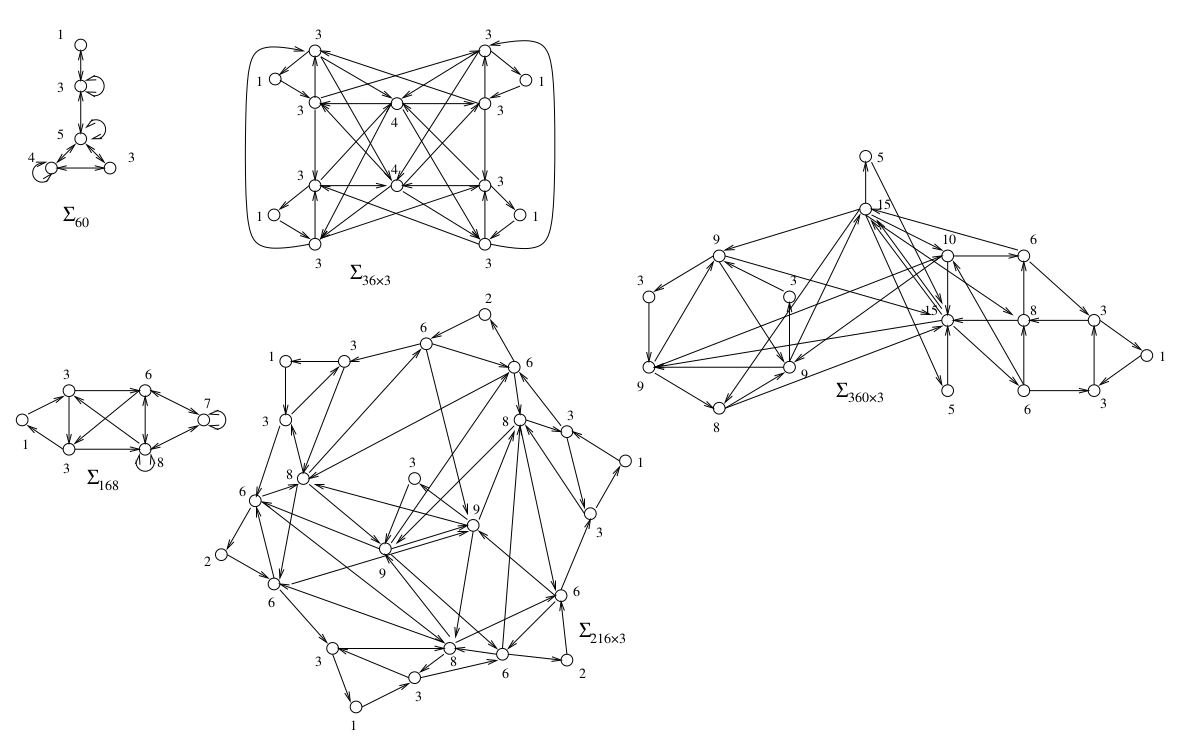
\includegraphics[scale=0.4]{Pictures/SU3finitequivers.png}
            \caption{Quivers of the exceptional finite subgroups of $\SU(3)$.}
        \end{figure}

    \subsection{$S=\C^3/(\Z_m\times\Z_n)$}

        \subsubsection{Representations of $\Z_m\times\Z_n$}

           We consider the group $\Z_m\times\Z_n$. Let us denote by $\{\mu_i\}_{i=0,\dots,m-1}$ and $\{\sigma_j\}_{j=0,\dots,n-1}$ two complete set of irreducible representation of $\Z_m$ and $\Z_n$ respectively, with
           \begin{align}
               \mu(g_1)&=\zeta^i_m\\
               \sigma_j(g_2)&=\zeta^j_n
           \end{align}
           where $g_1$ and $g_2$ are the generating elements of $\Z_m$ and $\Z_n$ respectively. $\Z_m\times\Z_n$ is of order $mn$ and possesses the same number of equivalency classes (abelian). It has therefore $mn$ irreducible representations. Since the group is abelian, they are all of dimension $1$. Let us denote by $\{T_k\}_{k=0,\dots,m+n-1}$ a complete set of irreducible representations. Since we have a product group, for any $k$ there exists indices $i(k)$ and $j(k)$ such that $T_k=\mu_{i(k)}\otimes\sigma_{j(k)}$. We choose the indices $i(k)$ and $j(k)$ such that
           \begin{align*}
               T_0 &= \mu_0\otimes\mu_0,\\
               T_1 &= \mu_0\otimes\mu_1,\\
               T_2 &= \mu_0\otimes\mu_2,\\
               &\vdots\\
               T_{n-1} &= \mu_0\otimes\mu_{n-1},\\
               T_n &= \mu_1\otimes\mu_0,\\
               &\vdots\\
               T_{2n-1} &= \mu_1\otimes\mu_{n-1},\\
               &\vdots\\
               T_{mn-1} &= \mu_{m-1}\otimes\mu_{n-1}.
           \end{align*}
           That is, we take
           \begin{equation}
               \begin{cases}
                   i(k) &= \lfloor k/n\rfloor\\
                   j(k) &= k\mod n
               \end{cases}\qquad \Leftrightarrow \qquad k=i(k)n+j(k).
           \end{equation}
           Note that this simply a dictionary between a line notation and a matrix notation and that it is indeed a bijection $k\Leftrightarrow i,j$. In this way, we can proceed to similar manipulations than before, were we used line notations. 

           Any representation $R$ of $\Z_m\times\Z_n$ can be decomposed as
           \begin{equation}
               R=\bigoplus_{i,j}N_k T_k=\bigoplus_{i,j}N_{ij}(\mu_{i}\otimes\sigma_{j})
           \end{equation}
           with $N_k=N_{i(k)j(k)}$. We must have $\sum_kN_k=3$. In other words, any representation of $\Z_m\times\Z_n$ on $\C^3$ is equivalent to
           \begin{equation}
                R(g_1,g_2)=[(\mu_{a}\otimes\sigma_{a'})\oplus(\mu_{b'}\otimes\sigma_{b'})\oplus(\mu_{c}\otimes\sigma_{c'})](g_1,g_2)=
               \begin{bmatrix}
                   \xi^a_m\xi^{a'}_n & 0 & 0 \\
                   0 & \xi^b_m\xi^{b'}_n & 0 \\
                   0 & 0 & \xi^c_m\xi^{c'}_n
               \end{bmatrix}.
           \end{equation}
           The determinant condition is
           \begin{align}
                \xi^{a+b+c}_m &= \xi^{-a'-b'-c'}_n\\
               \Leftrightarrow (a+b+c)\mod m &= (a'+b'+c')\mod n
           \end{align}

           

           \begin{equation}
            R(g_1,g_2)=
           \begin{bmatrix}
               \xi_m & 0 & 0 \\
               0 & \xi_n & 0 \\
               0 & 0 & \xi^{-1}_m\xi^{-1}_n
           \end{bmatrix}.
       \end{equation}

    \subsubsection{Projection}

        Let us start by the gauge field. We consider a unitary representation $(\rho,\C^N)$ of $\Z_m\times \Z_n$ on $\C^n$ and decompose it as
        \begin{equation}
            \rho=\bigoplus_{i,j}N_k T_k
        \end{equation}
        such that
        \begin{equation}
            \rho(g)=
            \begin{bmatrix}
                T_0(g) & & & \cdots & & & 0 \\
                & \ddots & & & & & \\
                & & T_0(g) & & & &  \\
                \vdots & & & \ddots & & & \vdots \\
                & & & & T_{mn-1}(g) & & \\
                & & & & & \ddots & \\
                0 & & & \cdots & & & T_{mn-1}(g) 
            \end{bmatrix}
            \hspace{-0.2cm}
            \begin{tabular}{l}
            $\left.\lefteqn{\phantom{
                \begin{matrix}
                    a_0\\ \ddots\\ a_0\ 
                \end{matrix} 
            }}\right\}N_0$\\
            \vdots \\
            $\left.\lefteqn{\phantom{
                \begin{matrix}
                    b_0\\ \ddots\\ b_0\ 
                \end{matrix}
            }} \right\}N_{mn-1}$
            \end{tabular}.
        \end{equation}

        We can now use our usual bi-index notation $A_{\mu;k\alpha_k,l\beta_l}$ with $k,l=0,\dots mn-1$ and $\alpha_k,\beta_k=0,\dots,N_k$ but instead it is more convenient to come back to our matrix notation by writing the block $A_{\mu;k,l}$ as $A_{\mu;i(k)j(k),i(l)j(l)}$ that we simply denote by $A_{\mu;ij,i'j'}$ with $i,i'\in\{0,\dots,n-1\}$ and $j,j'\in\{0,\dots,n-1\}$. So for $m=2,n=3$ for example, the link between the two notations is
        {\tiny
        \begin{equation}
            \begin{bmatrix}
                A_{\mu;00} & A_{\mu;01} & A_{\mu;02} & A_{\mu;03} & A_{\mu;04} & A_{\mu;05} \\
                A_{\mu;10} & A_{\mu;11} & A_{\mu;12} & A_{\mu;13} & A_{\mu;14} & A_{\mu;05} \\
                A_{\mu;20} & A_{\mu;21} & A_{\mu;22} & A_{\mu;23} & A_{\mu;24} & A_{\mu;05} \\
                A_{\mu;30} & A_{\mu;31} & A_{\mu;32} & A_{\mu;33} & A_{\mu;34} & A_{\mu;05} \\
                A_{\mu;40} & A_{\mu;41} & A_{\mu;42} & A_{\mu;43} & A_{\mu;44} & A_{\mu;05} \\
                A_{\mu;50} & A_{\mu;51} & A_{\mu;52} & A_{\mu;53} & A_{\mu;54} & A_{\mu;05}
            \end{bmatrix}=
            \begin{bmatrix}
                \begin{bmatrix}
                    A_{\mu;00,00} & A_{\mu;00,01} & A_{\mu;00,02}\\
                    A_{\mu;01,00} & A_{\mu;01,01} & A_{\mu;01,02}\\
                    A_{\mu;02,00} & A_{\mu;02,01} & A_{\mu;02,02}\\
                \end{bmatrix}
                \begin{bmatrix}
                    A_{\mu;00,10} & A_{\mu;00,11} & A_{\mu;00,12}\\
                    A_{\mu;01,10} & A_{\mu;01,11} & A_{\mu;01,12}\\
                    A_{\mu;02,10} & A_{\mu;02,11} & A_{\mu;02,12}\\
                \end{bmatrix}\\
                \begin{bmatrix}
                    A_{\mu;10,00} & A_{\mu;10,01} & A_{\mu;10,02}\\
                    A_{\mu;11,00} & A_{\mu;11,01} & A_{\mu;11,02}\\
                    A_{\mu;12,00} & A_{\mu;12,01} & A_{\mu;12,02}\\
                \end{bmatrix}
                \begin{bmatrix}
                A_{\mu;10,10} & A_{\mu;10,11} & A_{\mu;10,12}\\
                A_{\mu;11,10} & A_{\mu;11,11} & A_{\mu;11,12}\\
                A_{\mu;12,10} & A_{\mu;12,11} & A_{\mu;12,12}\\
            \end{bmatrix}
            \end{bmatrix}
        \end{equation}}
        So instead of considering $A_\mu$ to be a single $mn\times mn$ matrix of element $A_{\mu;kl}$, where $A_{\mu;kl}$ are $N_k\times N_l$ matrices, we consider it as an $m\times m$ where each element $A_{\mu,ii'}$ (line $i$ column $i'$) is itself an $n\times n$ matrices with elements $A_{\mu;ij,i'j'}$ (line $j$ column $j'$), as shown above.

        Using these notations, the gauge field transforms as
        \begin{equation}
            A_{\mu;ij,i'j'} \mapsto (\mu_i(g)\otimes\sigma_j(g))A_{\mu;ij,i'j'}(\mu_{i'}(g)\otimes\sigma_{j'}(g))^{-1} = \zeta^{i-i'}_m\zeta^{j'-j}_n A_{\mu;ij,i'j'}
        \end{equation}
        so invariant configurations can possess non-vanishing components $A_{\mu;ij,i'j'}$ only if
        \begin{align}
            \zeta^{i-i'}_m &= \zeta(j'-j)_n \\
            \Leftrightarrow\quad (i-i')\mod m &= (j'-j)\mod n \\
            \Leftrightarrow\quad j' &= j+\abs{i'-i}.
        \end{align}
        This means that the submatrices $A_{\mu;ii'}$ has an off-diagonal block form with offset $\abs{i'-i}$. Once again, for a general $n$, the difficulty is only computational, not conceptual. This can therefore easily be implemented into Mathematica and we get the form of the gauge field for any $n$.

        For the scalar fields, we have
        \begin{align}
            X^m_{ij,i'j'}&\mapsto R(g)\indices{^m_n}(\mu_i(g)\otimes\sigma_j(g))X^n_{ij,i'j'}(\mu_{i'}(g)\otimes\sigma_{j'}(g))^{-1}\\
            &\quad =
            \begin{cases}
                \zeta^{i-i'+1}_m\zeta^{j-j'}_n X^m_{ij,i'j'},\qquad m=0,1\\
                \zeta^{i-i'}_m\zeta^{j-j'+1}_n X^m_{ij,i'j'},\qquad m=2,3\\
                \zeta^{i-i'-1}_m\zeta^{j-j'-1}_n X^m_{ij,i'j'},\qquad m=4,5.
            \end{cases}
        \end{align}
        So a configuration is invariant if and only if the only non-vanishing component satisfy
        \begin{align}
            m=0,1 &: (i-i'+1)\mod m = (j'-j)\mod n\\
            m=2,3 &: (i-i')\mod m = (j'-j-1)\mod n\\
            m=4,5 &: (i-i'-1)\mod m = (j'-j+1)\mod n.
        \end{align}

\section{Summary of orbifold worldvolume theories}

    \begin{table}[H]
        \centering
        $
        \begin{array}{|c|c|c|}
            \hline
            \text{SUSY} & \Gamma & \text{Gauge group} \\ \hline
            \multirow{6}{*}{$\mN=2$} & \Z_{n} & (1^n) \\
            & \Z_{n}\times\Z_m & (1^{nm}) \\
            & \D_{n} & (1^4,2^{n-3}) \\
            & \mathcal{T} & (1^3,2^3,3) \\
            & \mathcal{O} & (1^2,2^2,3^2,4) \\
            & \mathcal{I} & (1,2^2,3^2,4^2,5,6) \\ \hline
            \multirow{11}{*}{$\mN=1$} & T & (1^3,3) \\
            & O & (1,2^2,3^2) \\
            & I & (1,3^2,4,5) \\
            & \Delta_{3n^2} (n=0\mod 3) & (1^9,3^{\frac{n^2}{3}-1}) \\
            & \Delta_{3n^2} (n\neq0\mod 3) & (1^3,3^{\frac{n^2-1}{3}}) \\
            & \Delta_{6n^2} (n\neq0\mod 3) & (1^2,2,3^{(2n-1)},6^{\frac{n^2-3n+2}{6}}) \\
            & \Sigma_{168} & (1,3^2,6,7,8) \\
            & \Sigma_{216} & (1^3,2^3,3,8^3) \\
            & \Sigma_{36\times 3} & (1^4,3^8,4^2) \\
            & \Sigma_{216\times 3} & (1^3,2^3,3^7,6^6,8^3,9^2) \\
            & \Sigma_{360\times 3} & (1,3^4,5^2,6^2,8^2,9^3,10,15^2) \\ \hline
        \end{array}
        $
        \caption{All supersymmetric orbifold worldvolume theories.}
    \end{table}

\section{Finite orbifold quiver gauge theories}

    For any QFT, the Callan-Symanzik equations dictates the behavior, under the renormalization group flow, of the $n$-point correlator $G^{(n)}(\{\phi(x_i)\};M,\lambda)$ forthe quantum fields $\phi(x)$ according the the renormalizationof the coupling $\lambda$ and momentum scale $M$:
    \begin{equation}
        \left[M\pdv{}{M}+\beta(\lambda)\pdv{}{\lambda}+n\gamma(\lambda)\right]G^{(n)}(\{\phi(x_i)\};M,\lambda)=0,
    \end{equation}
    where the dimensionless functions $\beta$ and $\gamma$ are the $\beta$-function and the anomalous dimension respectively. As usuall, the determine how the shifts $\lambda\to\lambda+\delta\lambda$ in the coupling constant and $\phi(1+\delta\eta)\phi$ in the wave function compensate for the shift in the renomalization scale $M$:
    \begin{equation}
        \beta(\lambda)\equiv M\pdv{\lambda}{M},\qquad \gamma(\lambda)\equiv-M\pdv{\eta}{M}.
    \end{equation}
    Thee are three possible behaviours for the $\beta$-function when $\lambda$ is small: $\beta(\lambda)>0$ then the theory has good IR behaviour and admits valid Feynman permutation theory at large distances, $\beta(\lambda)<0$ then the theory is asymptotically free and has a good permutative behaviour in the UV limit and finally if $\beta(\lambda)=0$ then the coupling constants do not flow and the renormalized couplings are always equal to the bare ones.

    Theories in which no divergences can be associated with the coupling in the ultraviolet are called \emph{finite} theories. To find such theories, supersymmetry is often a very god tool as it indices cancellation of the boon-fermion loop effects. More precisely, $\mN=4$ SYM have been shown to be finite to all orders, for $\mN=2$ SYM it has been shown that no higher than $1$-loop corrections exist for the $\beta$-function (Adler-Bardeen theorem) and for $\mN=1$ theories the vanishing at $1$-loop implies the vanishing at $2$-loops. Finite non-supersymmetric theories has however also been porposed (see \cite{He:2018gvd} for references). Of particular interest are theories which, in addition to a vanishing $\beta$-function, also have a vanishing anomalous dimensions. These theories are often part of a continuous manifold of scale-invariant theories and are characterized by the existence of exactly marginal operators (and hence dimensionless coupling constants). An important result is that there is a choice of coupling constant such that both the $\beta$-function and the anomalous dimensions vanish at first order, then the theory is necessarily finite at all orders.

    From \eqref{eq:defaij}, we must have
    \begin{equation}
        \dim(\mR)r_i=\sum_{j\in I}a^{\mR}_{ij}r_j.
    \end{equation}
    with $r_i\equiv\dim\rho_i$. It was shown (see \ref{He:2018gvd} for references) that this equation necessitates the vanishing of the $1$-loop $\beta$-function. In addition, we discussed that the remaining SUSY must be in the commutant of $\Gamma$ in $\SU(4)$ R-symmetry of the $\mN=4$ parent theory. It was shown in \cite{vafa1998,https://doi.org/10.48550/arxiv.hep-th/9706110} that the $1$-loop $\beta$-function is proportional to the function $dr_i-a^d_{ij}r_j$, called the \emph{discriminant function}:
    \begin{equation*}
        \beta_{1\text{-loop}}\propto dr_i-a^d_{ij}r_j,\qquad d\equiv 4-\mN.
    \end{equation*}
    Since the vanishing of the $\beta$-function signifies finitude, we have in particular the following necessary conditions for finitude:
    \begin{equation*}
        \begin{array}{c|c}
            \text{SUSY} & \text{Finitude} \\ \hline
            \mN=2 & 2r_i = a^2_{ij}r_j \\
            \mN=1 & 3r_i = a^3_{ij}r_j \\
            \mN=0 & 4r_i = a^4_{ij}r_j \\
        \end{array}
    \end{equation*}
    Note that in the case $\mN=2$ this condition is necessary and sufficient but not for $\mN=1$ and $\mN=0$ where one also have to chack the superpotential. In the non-supersymmetric case, vanishing of the $1$-loop $\beta$-function does not necessarily implies the vanishing of the following orders so we consider the notion finiteness in a weaker sense where only the leading order must vanish.

    Finitude of quiver gauge theories constrcuted in from D-brane probing singularities, the Hanany-Witten setup or geometric engineering is very much linked the the mathematical properties of their quiver. See \cite{Hanany:1999sp} for more details.
    

\section{Classical McKay correspondence from strings}

    We mentionned before the equivalence between fractional branes stuck at orbifold singularities and wrapped branes on the blow-up resolution. From the point of view of the worldvolume theory, this equivalence is exhibited by going from the Higgs branch to the Coulomb branch. The first step to understand this was done by Kronheimer. He showed that the resolution of the orbifold $\C^2/\Gamma$ with $\Gamma$ a finite group of $\SU(2)$ is precisely the generic form of the gauge orbit of the direct product of $\U(N_i)$ factors. From the QGT point of view, the product of those circle group is the gauge group of the theory and each factor is associated to a vertex of the quiver. The fields of the theory are organized as a linear representation into a direct sum of $\Hom(V_i,V_j)$ for each edge. If we pick one field and follow it around as the gauge group transforms it, the space swept out is the gauge orbit of that field. Kronheimer then showed that, if the quiver is a Dynkin diagram, this orbit is $\C^2/\Gamma$. 
    
    Now in general, gauge theories with with simple Lie groups (such as $\SU(N), E_8,$etc) are more interesting than the ones with gauge groups that are direct products so how could we relate the two? The mechanism the relates the two classes of theories is SSB, or \emph{Higgsing}. Indeed, one may embed the fields configurations in a higher-dimensional field configuration space (see them as submatrices of bigger matrices) on which acts the bigger (simple) Lie group. To from this group to a product of small ones. Fixing this submatrix-structure then singles out every gauge group factor one by one as the stabilizer subgroups of every submatrix. The final step is $\mN=2$ super Yang-Mills theories (Seiberg-Witten theory) which have a potential such that its vacua (more precisely the Higgs branch part) break a simple Lie group down to a Dynkin diagram QGT. The Coulomb branch is supposed to behave in a similar way. To summarize, the relation between simple Lie groups and the finite subgroups of $\SU(2)$ is the following:
    \begin{enumerate}
        \item start with $\mN=2$ SYM with gauge group that is a simple Lie group,
        \item let it spontaneously find its vacuum,
        \item consider the orbit space of the remaining spontaneously broken symmetry group,
        \item the latter space is the resolution of the orbifold of $\C^2/\Gamma$.
    \end{enumerate}

    All the details are presented in \cite{albertssonthesis}.

\section{A note about projective representations, discrete torsion and deformations}

    \subsection{Projective representations and discrete torsion}

        Up until now, and in particular in all of our computations in section \ref{sec:orbsing}, we only considered ordinary representations, i.e. linear representations. We can however use a more general representations such as projective representations for example. That is, representations $\rho$ of $\Gamma$ such that for all $\gamma_1,\gamma_2\in\Gamma$,
        \begin{equation}
            \rho(\gamma_1)\rho(\gamma_2)=A(g_1,g_2)\rho(\gamma_1\gamma_2)
        \end{equation}
        for some factor $A(\gamma_1,\gamma_2)$. The $A(\gamma_1,\gamma_2)=1$ corresponding to linear representations. For consistency reasons, the factor $A(g_1,g_2)$ cannot be completely arbitrary and must a cocycle condition. As a result, the possibilities for $A(\gamma_1,\gamma_2)$ are classified by the second cohomology group $H^2(\Gamma,\C^*)$, also called \emph{discrete torsion}. There exists a projective representation if and only if the latter does not vanish. This new liberty, whenever admissible, provides new classes of quiver gauge theories that can be remarkably different from the ones we considered up until now, with no discrete torsion.

        What happens is that if one turns on an NSNS B-fiels alors the worldvolume, then the moduli space is expected to a non-commutative version of a Calabi-Yau space. This haw the discrete torsion is physically realized. Another, and actually equivalent through T-duality, way of studying gauge theories is to consider D-branes streched between configurations of NS$5$-branes\footnote{D$5$-branes are charged under the Ramond-Ramond field whose quanta comes from the Ramond-Ramond sector but NS$5$-branes are charges under the Kalb-Ramonf field whose quanta comes fromthe Neveu-Schwarz. On the worldvolume of an NS$5$-brane (6-dimensional) propagates propagates a superstring, this called the \emph{little string}.}. This is the\emph{Hanany-Witten setup}.

        The discrete tosrion also appears when writing the full open strin gpartition function that inclues the twisted sector where there is ambiguity up to a phase factor. As a consequence from modular invariance, the latter must satisfy certain cocycle conditions. It is precisely the deiscrete torsion. Note that this has been found to be true only for the open string sector.

    \subsection{Quiver gauge theories deformations and conifold}

        We can deforming the singular algebraic description of the orbifold with a field into a family smooth surfaces. The resulting total space is the \emph{conifold}.